\documentclass{acm_proc_article-sp}
\usepackage[colorlinks,linkcolor=red,anchorcolor=blue,citecolor=green,urlcolor=black]{hyperref}
\usepackage{epsfig}
\usepackage{breqn}


\newcommand{\comments}[1]{}

\begin{document}

%\title{Deduplication Localization for Virtual Machine Snapshot Backup}
\title{Collocated Deduplication with Fault Isolation for Virtual Machine Snapshot Backup}
%\title{BigArchive: Low-cost and Scalable Deduplication Storage for VM Snapshot}



\author{
Wei Zhang, Michael Agun,  Tao Yang \\
%Wei Zhang$^{\star}$, Michael Agun,  Tao Yang$^\star$
%{\normalsize$^\star$  University of California at Santa Barbara}, {\normalsize$^\dagger$Alibaba Inc.}
%Wei Zhang, Tao Yang, Gautham Narayanasamy\\
Department of Computer Science\\
University of California at Santa Barbara
%\and
%Hong Tang\\
%Alibaba Inc.
}
%, Gautham Narayanasamy$^\star$, and Hong Tang$^\dagger$ \\



\maketitle

\begin{abstract}
%Virtualization has became the engine behind many cloud computing platforms.
In a virtualized cloud cluster, frequent  snapshot backup of virtual disks improves
hosting  reliability; however, it  takes significant 
memory resource to perform data duplication in order to remove
excessive redundancy among snapshots.
This paper presents a low-cost deduplication solution scalable for a large number 
of virtual machines.  The key idea is to separate duplicate detection from 
the actual storage data backup instead of using inline deduplication, and partition
global index and  detection requests among machines using  fingerprint values.
Then each machine conducts duplicate pre-detection partition by partition independently with a minimal memory usage.
%in parallel among all machines and  each machine full duplication detection is 
Another optimization is to allocate and control
buffer space for exchanging  detection requests and duplicate summary among machines.
%The memory requirement and disk usage for the proposed solution is very small while the overall thoughput
%and backup process timing is not compromised. 
Our experiments show that  the proposed multi-phase scheme 
uses a very small amount of system resources while delivering a satisfactory backup throughput.
%in a large cloud setting.
%which only reqiires a very small amount of memory and CPU resource.  
%Experimental results  show the proposed scheme  can achieve high deduplication ratio while using
%a  small  amount of cloud resources. 

%Our system compares well with Amazon Glacier, in that, both of them are low-cost archival systems, 
%supporting lazy storage with asynchronous notification mechanisms and achieve parallelism by 
%reading/writing from multiple storage nodes/disks simultaneously. At the same time, 


%While dirtybit-based technique can identify unmodified data between versions, 
%full deduplication with fingerprint comparison  can remove more redundant content
%at the cost of computing resources.
%with  for similarity comparison and   reliability handling.
%Current snapshot deduplication is mainly done through copy-on-write 
%on fixed-size disk blocks. Such solutions cannot handle the
% cross VM data duplication because VMs do not share any data. 
%In addition, storing VM images and their snapshots
%in the same storage engine reduce the underline design flexibility because 
%these two kinds of data have distinct access requirements.
%In this paper, 
%we show that there is a large amount of duplicated data shared amongy virtual machines
%through a production VM data study and thus it is expective to perform cross-machine deduplication. 
% first perform a large scale study in production VM clusters 
%to show that cross VM data duplication is severe due to they have large amount of
%common data. Then our data analysis finds out that the overall data duplication pattern follows the Zipf's law.
%Base on these discoveries, we propose a snapshot storage deduplication scheme using variable-size chunking
%to address the above problem efficiently.
%We eliminate the majority of cross VM data duplication by pre-select
%a small set of frequently seen data blocks to be shared globally, and we also remove
%many cross snapshot duplication by using smaller chunking granuarity and locality.
\end{abstract}
%\begin{IEEEkeywords}
%Cloud storage backup,  Virtual machine snapshots,  Distributed data deduplication
%\end{IEEEkeywords}


% A category with the (minimum) three required fields
\category{H.4}{Information Systems Applications}{Miscellaneous}
%A category including the fourth, optional field follows...
\category{D.2.8}{Software Engineering}{Metrics}[complexity measures, performance measures]

\terms{Theory}

\keywords{ACM proceedings, \LaTeX, text tagging} % NOT required for Proceedings

\section{Introduction}
In a cluster-based cloud environment such as ones provided by Amazon EC2\cite{AmazonEC2} 
and Alibaba Aliyun\cite{Aliyun},
each physical machine runs a number  of virtual machines as  instances of a guest operating system 
and their  virtual hard disks are represented as virtual disk image files in the host operating system.
%virtual disk image files (e.g. .vhd, .vmdk) in the host operating system.
%Backup  of virtual disks is relatively straightforward since
%these image files are stored as regular files from the external point of view,
%backing up VM's data is mainly done by taking snapshots of virtual disk images.

%A snapshot preserves the data of a VM's file system at a specific point in time. 
%VM snapshots can be  backed up  incrementally by comparing blocks from one version to another 
%and only the blocks that have changed from the previous version of snapshot will be saved~\cite{Clements2009,Vrable2009}. 
Frequent  snapshot backup of virtual disk images  can increase  the service reliability. 
For example, the Aliyun cloud , which is  the largest cloud service provider by Alibaba in China, 
automatically conducts  the backup of virtual disk images to all active users every day.
The cost of supporting a large number of concurrent backup streams is high
because of the huge storage demand and  
Using a separate  backup service with full deduplication support~\cite{venti02,bottleneck08}
can effectively identify content duplicates among snapshots and  remove 
redundant storage content,  but the solution can be expensive and there is a large amount of 
network traffic to transfer  data from the host machines to the backup facility
before duplicates are removed.


This paper seeks for a low-cost architecture option and considers that
a backup service collocates  on  the cloud cluster with a minimum resource usage. 
%Since most of backup data is not used in practice, system resource in such a service is not fully utilized.
The dirty bit approach~\cite{??}  which checks the version difference can effectively remove
duplicates while using content fingerprints can significantly compress more~\cite{Bottlneck08}.
On the other hand, comparing fingerprints  adds significant  memory cost. 
Since each physical machine in a cluster  hosts many VMs, memory contention happens frequently.
Cloud providers often wish that the backup service only consumes  small or modest resources
with a minimal impact to the existing cloud services.  A 
recent study using subsampling~\cite{Guo2011}  can significantly reduce the memory requirement.
Another issue is that after deduplication, the most of data blocks are shared by many virtual machines.
Failure of such blocks would  have a catastrophic effect and many snapshots of virtual machines would be affected.
Furthermore, 
%that deletion of old snapshots compete for computing resource as well. That is because data dependence created
deletion of old snapshots compete for computing resource as well and that  needs
to be considered. That is  because data dependence created
by duplicate relationship among snapshots  adds processing complexity.
% especially when  VMs can migrate around in the cloud.

The paper proposes an integrated approach which uses  multiple duplicate detection strategies
integrating  version  detection, small-scope inner VM duplicate comparison
and controlled cross-VM comparison. 
The key idea of this approach is to localize duplicate detection within each virtual machine as much as possible
and minimize memory usage while delivering a decent deduplication efficiency. 
That brings the benefits for parallelism  utilization and fault isolation.
Our deletion strategy uses a double Boomer filer strategy for periodic mark-and-sweeping of expired data blocks.
We have developed a prototype system that runs a cluster of Linux machines running Zen.
The backup storage uses a standard distributed file system  with data replication and
we allocate more  replicas for the commonly-shared  data blocks among VM snapshots to enhance fault tolerance.



%************** Paper sections summary
%THIS NEEDS MODIFICATION
The rest of this paper is organized as follows.
Section~\ref{review} reviews background and related work.
Section~\ref{sec:framework}  discusses the  design framework and system architecture.
Section~\ref{sec:model}  analyzes the benefit of our approach for fault isolation. 
Section~\ref{exper} is our experimental evaluation that compare with the other approach.
Section~\ref{conc}  concludes this paper.

%We are seeking Unlike the previous work dealing with general file-level backup and deduplication, our problem is focused on 
%virtual disk image backup. Although we treat each virtual disk  as a file logically, its size is very large.
%On the other hand, we need to support parallel backup of a large number of virtual disks in a cloud every day. 
%One key requirement we face at Alibaba Aliyun is that VM snapshot backup should only use a minimal amount of system
%resources so that most of resources is kept for regular cloud system services or applications.
%Thus our objective is to exploit the characteristics of VM snapshot data and
%pursue a cost-effective deduplication solution. 
%Another goal  is to decentralize VM snapshot backup and  localize  deduplication as much as possible,

%,extreme_binning09,sparseindex09
\comments{
By observations on the VM snapshot data from production cloud, we found snapshot data duplication 
can be easily classified into two categories: \emph{inner-VM} and \emph{cross-VM}. Inner-VM duplication
exists between VM's snapshots, because the majority of data are unchanged during each backup period. 
On the other hand, Cross-VM duplication is mainly due to widely-used software and libraries such as Linux and MySQL.
As the result, different VMs tend to backup large amount of highly similar data.

With these in mind, we  have developed a distributed multi-level solution to conduct 
segment-level  and block-level inner-VM  deduplication to localize the deduplication effort when possible.
It then makes cross-VM deduplication by excluding a small number of
popular common data blocks from being backed up. Our study shows that common data blocks
occupy significant amount of storage space while they only take
a small amount of resources to deduplicate.
Separating deduplication into multi levels effectively accomplish the major space saving goal
compare the global complete deduplication scheme, at the same time it makes
the backup of different VMs to be independent for better fault tolerance.

The following table shows the strength and weakness of some well-know deduplication systems:
\begin{table}
    \begin{tabular}{|l|l|l|l|}
        \hline
        ~           & Scalability & Low-cost & Full Dedup \\ \hline
        DDFS        & N           & N        & Y          \\ 
        Ex-bin      & Y           & Y        & N          \\ 
        Guo         & Y           & N        & N          \\ 
        iDedup      & N           & Y        & N          \\ 
        Founadation & N           & N        & Y          \\
        \hline
    \end{tabular}
\end{table}
}

%\section{Design Overview}
In this section we briefly describe all the static things in our system, such like architecture, each component’s data structure, data locations, relationship of data references, etc.

We discuss the characteristics and 
main requirements for VM snapshot backup in a cloud environment.
which are different from a traditional data backup. 

\begin{enumerate}
\item {\em Cost consciousness.}
There are tens of thousands of VMs running on a large-scale cluster. 
The amount of data is so huge such that backup cost must be controlled carefully.
On the other hand, the computing resources allocated for snapshot service is very limited
because VM performance has higher priority.  
At Aliyun, it is required that while CPU and disk usage should be small or modest during backup time,
the memory footprint of snapshot service should not exceed 500MB at each node.

\item {\em Fast backup speed.}
Often a cloud has a few hours of light workload each day (e.g. midnight),  which creates an small window for automatic backup.
%But a  longer use of bandwidth and computing resource  for backup can create  noticeable  contention with the existing cloud,
%which is not preferred for cloud production system operation. 
Thus it is desirable that backup for all nodes
can be conducted in parallel and any centralized or cross-machine communication for
deduplication should not become a bottleneck.
%As a large-scale cluster hosting tens of thousand of active VMs everyday,  the amount of data
%to be processed is huge. 
%For example, in an Aliyun cluster with over 1,000 nodes and each hosts over 25 VMs, The aggreated amount of data 
 % the system must finish saving daily snapshots of all VMs in 2 hours. In our typical 1000 nodes cluster, each node hosts 25 VMs, each VM has 40GB of data on average, that translates to backup throughput of 139GB/second, or 500TB/hour.

% the system must finish saving daily snapshots of all VMs in 2 hours. In our typical 1000 nodes cluster, each node hosts 25 VMs, each VM has 40GB of data on average, that translates to backup throughput of 139GB/second, or 500TB/hour.
\item {\em Fault tolerance.}
The addition of data deduplication should not decrease the degree of
fault tolerance. It's not desirable that small scale of data failure affects the backup of many VMs.
%when users access snapshots in a recovery process. 
\end{enumerate}

There are multiple choices in designing a backup architecture  for VM snapshots.
We discuss the following design options with a consideration on their strengths and weakness.
\begin{enumerate}
\item  {\em An external and dedicated backup storage system.} 
In this architecture setting, a separate backup storage system using
the standard backup and deduplication techniques can be deployed~\cite{bottleneck08,extreme_binning09,sparseindex09}. 
This system is attached to the cloud network and every machine can periodically transfer snapshot data to 
the attached backup system. 
A key weakness of this approach is communication bottleneck between a large number of machines
in a cloud to this centralized  service.
Another weakness is that the cost of allocating separate resource for dedicated backup  can be expensive.
Since most of backup data is not used eventually, CPU and memory resource in such a backup cluster may not be fully utilized.
\item {\em A decentralized and co-hosted backup system with full deduplication.}
In this option, the backup system runs on an existing set of cluster machines.
% and a distributed storage architecture for backup allows a possible exploitation of  data locality between
%the source of data and storage location of backup data. 
The disadvantage is that 
%the backup service would compete CPU, memory, and disk resources with the other cloud services.
even such a  backup service may only use  a fraction of the existing disk storage, 
fingerprint-based search does require a significant amount of memory for fingerprint lookup of searching duplicates.
This competes memory resource  with the existing VMs.
%Decentralized deduplication is studied in ~\cite{Clements2009} and the focus is on
%block-level copy-on-write and compare-by-value techniques.

Even approximation~\cite{extreme_binning09,sparseindex09} can be used to reduce memory requirement,
one key weakness the hasn't been addressed by previous solutions is that global content sharing affects
fault isolation.
Because a content chunk is compared with a content signature collected from other users,
this artificially creates data dependency among different VM users.
% since storage for shared identical content chunks can become a failure point.
In large scale cloud, node failures happen at daily basis,
the loss of a shared block can affect many users whose snapshots share this 
data block. 
Without any control of such data sharing, we can only increase  
replication for global dataset to enhance the availability,
but this incurs significantly more cost.

%we want to isolate 
%each VM's snapshot backup as much as possible while still enjoy the benefit of deduplication.
%In large scale cloud, node faiures happen at daily basis, we don't want a problem at small scale
%to affect large amount of VMs due to data sharing.
%a key weakness of global content fingerprint comparison is that it affects fault isolation.

%2) data sharing among users for accessing common signagutes causes the system less resilient to storage failures.
%any loss of one piece of  shared data content hash and actualcontent will damange many VM snapshots, which can cause massive impacts
%on reliability of many users.

%Another point is that the previous work in signature-based comparison does not address
%load balancing for a distributed environment during parallel access.  
%Some content signatures can be extremely hot, but the machines  that  handle such signatures can become
% a bottleneck. Uncoordinated signature assignment could lead to imbalanced access workload.
\end{enumerate}


%There are multiple choices of snapshot backup design for VM images and our considerations are described
%as follows. 
%Our design considerations
%\begin{enumerate}
%\item {\bf Centralized vs. decenalized} 
%
%It is desirable to have  a decentralized architecture.
%Given a large amount of snapshot data communicated from each machine to the backup storage,
%with a distributed storage architecture for backup, one could exploit  exploit data locality between
%the source of data and storage location of data to reduce cross-platform bandwidth requirement for backup.

%execute in parallel and easy to coordinate. In fact, we want to avoid cross-node dependency at scheduling VM snapshot operations, such that no global coordinator is necessary.
%\item {Load balancing in resource consumption}: the cost of snapshot service shall be evenly distributed onto every node. We don't have a super powerful
%or stable node that can accept extra responsibility.
%\item {minimization of inter-user data dependency for fault tolerance}: we want to minimize the data dependency to a controllable level. Data deduplication means sharing of data, thus one failure at a single point may affect the snapshot service of hundreds of VMs, which is absolutely unacceptable.
%\item {Resource usage modeling and control}.
%\end{enumerate}

With these considerations in mind, we propose a decentralized backup architecture with multi-level and selective 
deduplication. This service is hosted   in the existing set of machines and resource usage is controlled
with a minimal impact to the existing applications.
The deduplication process is first conducted among snapshots within each VM
and then is conducted across VMs.  
Given the concern that searching duplicates across VMs is a global feature which can affect parallel performance
and complicate failure management,
we only eliminate the duplication of a small but popular data set while still maintaining a cost-effective deduplication ratio.
For this purpose, we exploit the data characteristics of snapshots and collect most popular data.
Data sharing across VMs is limited within this small data set such that adding replicas for it could enhance fault tolerance.
%
%in the  our studies show that there are a large amount of data unmodified in VM snapshots
%and shared among many users (e.g. OS data). The sharing pattern follows a zip-like distribution.
%With this characteristic, we can store a small amount of popular data items which coverage a large amount of
%snapshot data blocks. 
%We discuss our design and data analysis in the next section.


%This method is based on the observation of two facts in Aliyun's VM cloud: first, VM's OS disks contain 
%huge amount of operating system and software related data which is almost never modified during VM's life span. 
%Second, the duplication pattern of user generated data follows Zipf-like law, thus a tiny set of hottest data
%take up the majority of data duplication. As a result, if we extract these hot data as a common data set,
%then most of data duplication will emerge by searching in this very small scope.


%For example, In cloud storage, we are solving data deduplication problem in a different context of 
%data stream deduplication (the D2D case): our snapshot storage service is co-located with runtime VMs,
%thus we have very limited amount of system resource leave for data deduplication. For example,
%in Aliyun's 8-core, 48GB memory, 12TB VM server, there lives over 20 VMs who are hungrily competing for
%system resources: some may running map-reduce jobs, some may serving busy web requests, 
%some may storing backend databases, any behavior that affects user VMs performance or stability is unacceptable.

%To reduce the cost of deduplication, we must confine the scope of searching duplicates as much as possible,
%thus some hints are needed to tell us where the most likely duplicates would hide. 
%Several form of hints have been used in the past: many D2D systems exploits locality,
%which bases on the fact that duplicates are likely to appear in the same sequence as they have arrived before.
%Similarity is another popular hint, it suggests that two sets of data blocks may contain lots of
%duplicates if they are indetified as similar by certain similarity detection measurements.

Overall, our contributions are:
\begin{enumerate}
\item {\em CDS. parallelism, localized}
We designed a highly efficient global deduplication scheme using common data between VMs as the primary
deduplication target, which adopts to our resource-constrained production environment very well. We developed a fast
approxmation algorithm to extract the commonly used data from VM snapshot backups.

\item {\em Append Store.}
We address the problem of managing billions of small variable-sized data objects by building an append store
on top of our distributed file system (DFS). We carefully designed an efficient index data structure to 
optimize large sequential read/write requests, while minimize the cost of key to object location conversion.

\item {\em Fast Data Deletion.}
Traditional deletion in deduplication systems involves reference counting, either online or offline. Both ways
are costly due to the sharing of large amount of data objects.
We avoid this cost of data deletion with an approxmation deletion method using bloom filters.

\item {\em Fault-tolerant.}
Golbal deduplication brings data sharing across different users VM snapshots, therefore a single failure
on some data can break many VMs' snapshots. We avoid such all-to-all data dependency by restricting
the cross VM data sharing with the CDS. By taking extra care of protecting CDS data, 
the overall degree of fault tolerancy is guaranteed.

\end{enumerate}

\subsection{Design Considerations}
While this idea sounds conceptually simple, realizing it requires us to address three
significant challenges:
\begin{enumerate}
\item {\em In-cloud backup}
We decided to build 
\item {\em Inline deduplication}
Inline deduplication requires more resources and can suffer from latency issues as data is checked against metadata before being committed to disk or flagged as a duplicate.
\item {\em Data dependency}

\item {\em Backup speed}

\end{enumerate}
% \subsection{Architecture Overview}
% Our architecture is built on the Aliyun platform which provides the largest public VM cloud in China 
% based on Xen~\cite{Xen2003}. A typical VM cluster in our cloud environment
% consists of from hundreds to thousands of physical machines, each of which can
% host tens of VMs.

% A GFS-like distributed file system holds the responsibility of managing physical disk storage
% in the cloud. All data needed for VM services, which include runtime VM disk images and snapshot backup data,
% reside in this distributed file system.
% During the VM creation, a user chooses her flavor of OS distribution and the cloud system 
% copies the corresponding pre-configured base VM image to her VM as the OS disk, 
% and an empty data disk is created and mounted onto her VM as well. 
% All these virtual disks are represented as virtual machine image files in our
% underline runtime VM storage system. The runtime I/O between virtual machine and its virtual
% disks is tunneled by the virtual device driver (called TapDisk\cite{Warfield2005} at Xen). To avoid network latency and congestion, 
% our distributed file system place the primary replica of VM's 
% image files at physical machine of VM instance.
% During snapshot backup, concurrent disk write is logged 
% to ensure a consistent snapshot version is captured. 

% Figure~\ref{fig:arch} shows the architecture view of our snapshot service
% at each node. The snapshot broker provides the functional interface for  snapshot backup, access, and deletion.
% The inner-VM  deduplication is conducted by the broker to access meta data in the snapshot data store
% and we discuss this in details in Section~\ref{sect:innerVM}.
% The cross-VM deduplication is conducted by the broker to access 
% a common data set (CDS) (will discuss in Section~\ref{sect:crossVM},
% whose block hash index is stored in a distributed memory cache. 
% \begin{figure}[htbp]
%   \centering
%   %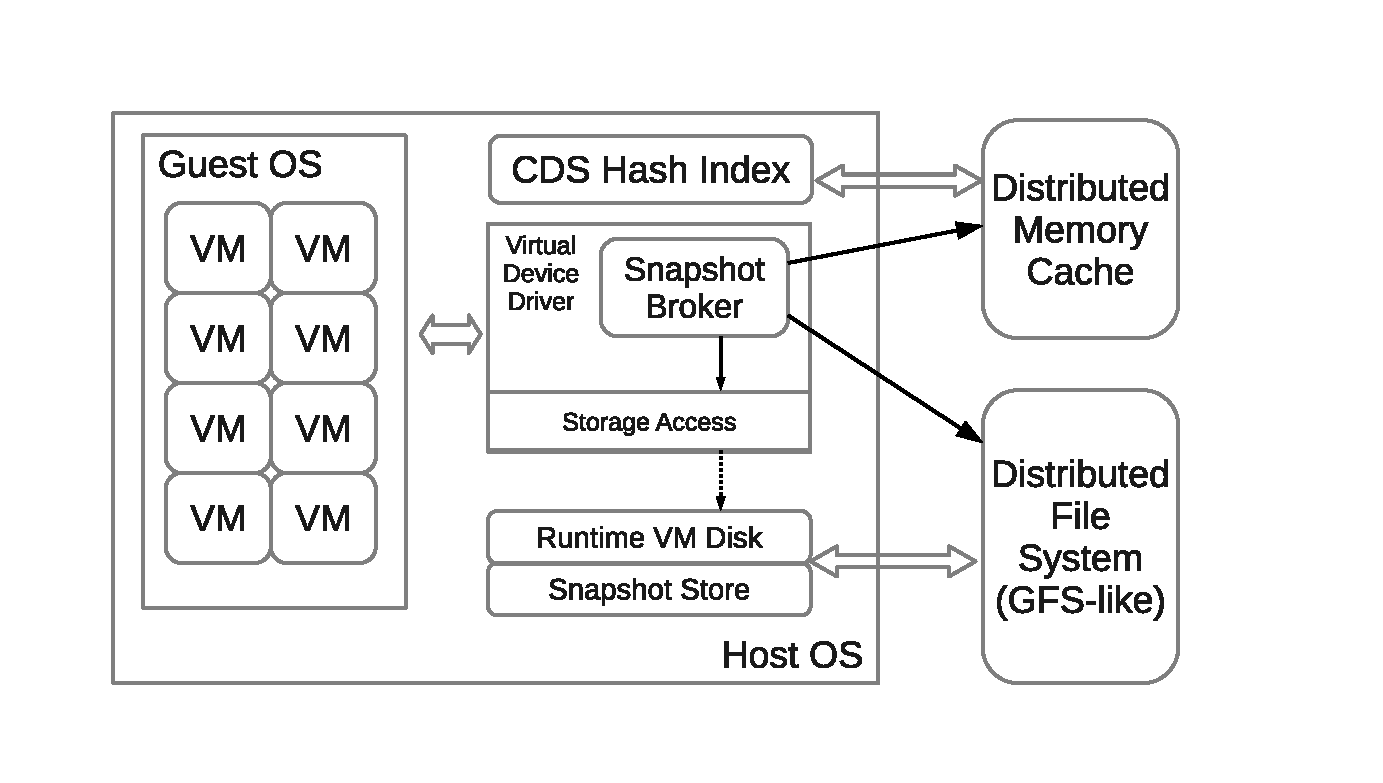
\epsfig{file=images/arch.eps, height=2in, width=2.66in}
%   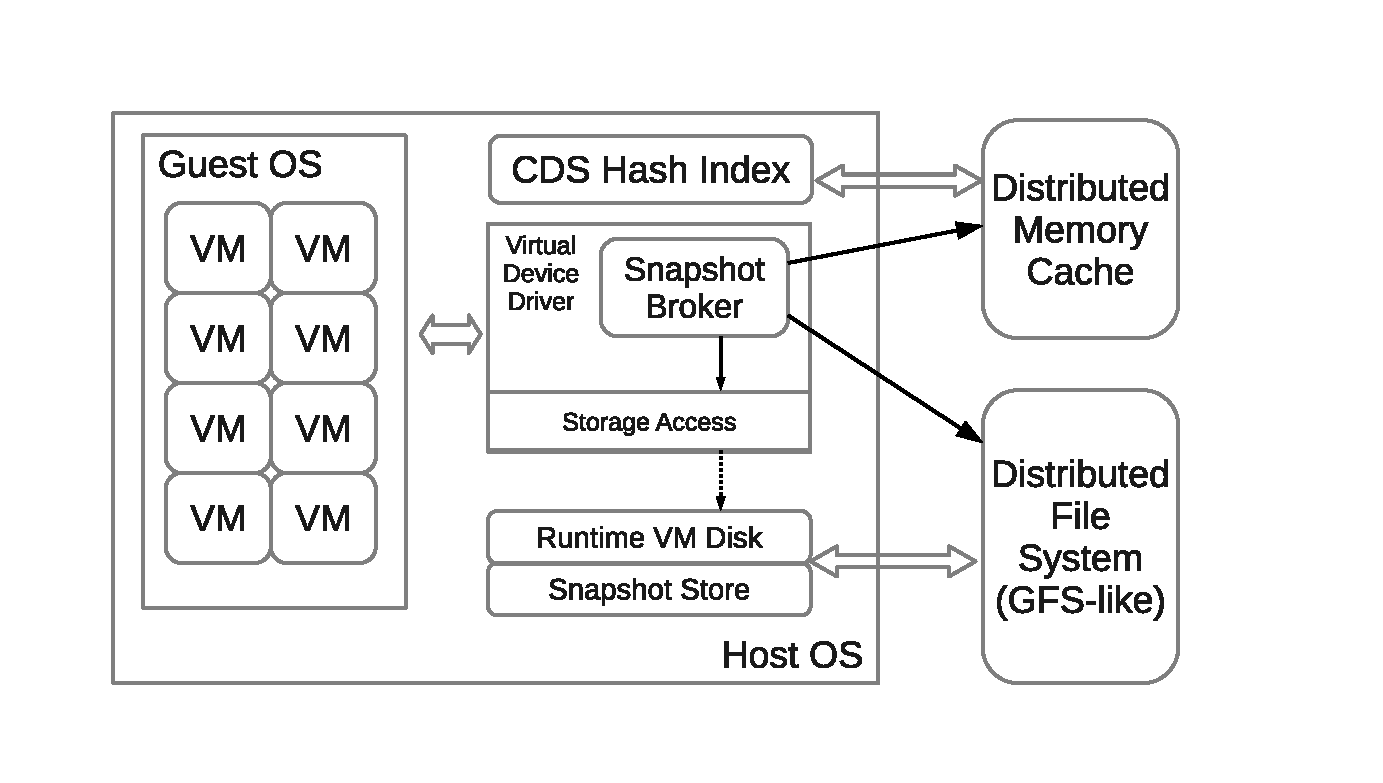
\epsfig{file=images/arch.eps, width=3.9in}
%   \caption{Snapshot backup architecture of each node.}
%   \label{fig:arch}
% \end{figure}
% The snapshot store 
% supports data access operations such as \emph{get}, \emph{put} and \emph{delete}.
% Other operations include data block traverse and resource usage report.
% The snapshot data does not need to be
% co-located with VM instances, and in fact they can even live in a different cluster to improve the 
% data reliability: when one cluster is not available, we are still able to restore its VMs from another cluster which
% holds its snapshot data. 
% %to reduce the impact to our users.
% %Get interface accepts a piece of data, write it to the underline data file, and return
% %a reference to the caller. This reference then can be used in the put interface to
% %retrive or delete the data, thus the caller of put interface must preserve the
% %data reference for future use. 
% %In addition to above standand data access operations, the snapshot service also supports
% %\emph{scan} and \emph{quota} methods. Scan allows us to traverse all the data blocks of each VM
% %in the snapshot store, and quota is used to acknowledge user how much space he
% %has actually used.

% Under the hood of snapshot store, it organizes and operates snapshot data 
% in the distributed file system. We let each virtual disk has its own snapshot store, 
% and no data is shared between
% any two snapshot stores, thus achieve great fault isolation. For those selected popular data
% that shared by many VM snapshot stores, we could easily increase its availability by having more replications.
% %Since all the underline data structures is append only,
% %upon a delete request, the corresponding data will only be marked rather than being deleted.
% %A compaction will take place when deleted data has accumulated to a certain threshold, thus 
% %reclaiming the disk space .


% \subsection{Block Storage Device}
\subsection{CDS}
Although locality based data reduction can remove most of the inner-VM duplications,
it's not able to solve the data duplication cross VMs. Different VMs still share large amount
of common data such that their snapshot backups would have a lot of data in common.
Our observations on Aliyun's real VM user data reveals several major sources of cross-VM data duplication:
  \begin{enumerate}
  \item \emph{System-related data}: These data are generated by public third-parties, they are copied/downloaded/installed into VM disks either automatically or manually. Once installed, operations on such data are mostly read only until software updates arrive. For example, data of operating systems, some widely-used software such as Apache and MySQL, and their documations all fall into this category.
  \item \emph{User-generated data}: These data are generated by individual user's behavior, either directly or indirectly. They are much less duplicated than the system-related data, but the zipf-like distribution indicates that a small amount of data in this category could represent most of data duplications.
  \item \emph{Zero-filled data}: Like previous studies [refs here], we've observed that zero-filled data exist pervasively at system wide. They are almost like the spaces and commas in text articles. Under content-based chunking, they were distilled as zero-filled blocks with the maximum allowed length. 
%Zero-filled blocks are mostly generated by user behavior to preserve the space for future data, thus we treat them as a special case of user-generated data.
  \end{enumerate}

Without eliminating the data duplication between VM snapshot backups, storage space is severely wasted when the number of VMs increases.
To address this problem, we developed a technique called \emph{Common Data Set (CDS)} to eliminate data duplication for all three situations above. 
CDS is a public data library that shared by all VM snapshot backups in the cluster, 
which consists of the most popular data blocks in VM snapshot backups. It is generated, 
managed and accessed in an uniform manner by all VMs such that [write some fancy system characteristic stuff here].

\subsection{CDS Size V.S. Coverage}
As a shared data library, we expect CDS to collect almost all the system related data, the most popular user-generated data and the zero-filled data block.
With CDS as a public data reference, each VM's snapshot backup has no need to store its own copies for data that can be found in CDS, instead they can just
store a reference.

The more data we put into CDS, the closer we come to complete deduplication. But in reality we are facing a list of restrictions such like [blabla].
We borrowed the idea of web caching[refs here] to analysis the size of CDS vesus its effectiveness on data reduction.

We let $M$ be the number of nodes in a cluster, $N$ be the number of VMs hosted per node,
and let $D$ denotes the average size of one VM's snapshot backups (after level 1 and 2 reduction, which is near 40 GB in our production environment).
And let $C_0$, $C_s$ and $C_u$ denote the size of zero-filled block, system-related data and user-generated data in CDS,
then the total size of CDS is represented by $C=C_0+C_s+C_u$.
We let $S_0$, $S_s$ and $S_u$ denote the corresponding data coverage ratio (with respect to $D$) by $C_0$, $C_s$ and $C_u$,
so the total space saving ratio is $S=S_0+S_s+S_u$.

Zero-filled block at maximum length is the first item we need to put into CDS. This is the one and only special data block, 
and because CDS only stores unique data blocks, $C_0$ is almost equal to 0. In practice we found zero-filled blocks account
for near 20\% of total data, so $S_0$ is 20\%.

The rarely modified system-related data are the second to be added to CDS. We have thousands of VMs in each cluster, 
but all these VMs fall into only a few OS types, using a limited selection of software, therefore data duplication in this category
is highly noticable in a global block counting. In particular, most of such data already exist in the VM base images. 
We analyzed VMs running various services from 7 mainstream OS types in our cluster, and found close to 50GB of such data in total. 
Because system-related data don't change frequently, it's safe to expect that for 20 OS variations 
and software updates in 2 years, $C_s$ will not grow to exceed 200 GB.
For each VM, from 2 to 20 GB of data can be reduced in this way, depends on the OS and service type, so on average we estimate
$S_s$ would be no less than 20\%.

The rest of data are user-generated, the total size of such data can be written as $D_u=D-S_0-S_s$, which is 60\% of $D$. 
It follows a zipf-like distribution with $\alpha$ between 0.65 to 0.7. 
Let $T_u$ be the total size of unique data blocks in $D_u$,
in practice we notice that complete deduplication for such data always result in a 2:1 reduction ratio,
, so $T_u=D_u/2$.
Since we collect the most popular user-generated data into CDS, the coverage of CDS on user-generated data
is $(C_u/T_u)^{1-\alpha}$.

The following table lists CDS coverage on user-generated data under different $\alpha$ and $C_u/T_u$.

[a table of coverage with alpha from 0.65-0.70, ratio from 0.002 0.005 0.01 0.02 0.05]

It's obviously that at least 30\% of user-generated data can be reduced in this way, using about 0.02 of $T_u$, or 0.01 of $D_u$.
The size of user-generated data in CDS would be 0.006$D$, with coverage $S_u=0.18D$.

Thus the estimation of CDS coverage is $S=S_0+S_s+S_u=0.58$, with the size of CDS to be no more than $(200 + 0.006*D*N)$ GB.
In a VM cluster of 100 machines, with 25 VMs on each physical machine, the size of CDS is 800 GB in total, or 8 GB per machine.
The total size of CDS index would be 8 GB, which will cost 80 MB memory on each machine. 

\subsection{Append Store}


\section{Background and Related Work}
\label{sect:background}


%In a virtualized cloud environment such as ones provided by Amazon EC2\cite{AmazonEC2} and Alibaba Aliyun\cite{Aliyun}, 
At a cloud cluster node, each instance of a guest operating system runs on a virtual machine, accessing virtual hard disks 
represented as virtual disk image files in the host operating system.
For VM snapshot backup, file-level semantics are normally not provided.
Snapshot operations take place at the virtual device driver level, which
means no fine-grained file system metadata can be used to determine the changed data. 
%Only raw access information at disk block level are provided. 
%Each physical machine hosts many VMs and petabytes of data in a cloud cluster need a frequent  backup. 
%Ideally speaking, snapshot backup must not affect the normal cloud service, which means that 
%only a very small slice of cluster resource can be used for the backup purpose.



The previous work for storage backup has extensively studied  data deduplication techniques can eliminate redundancy 
globally among different files from different users.
Backup systems have been developed to use content fingerprints to identify duplicate
content~\cite{venti02,Rhea2008}.  Offline deduplication is 
used in ~\cite{EMC,NetAppOffline} to remove previously written duplicates during idle time.
%,NGmiddleware2011}.
%Today's commercial data backup systems (e.g. from EMC and NetApp)
%\cite{emc_avamar}\cite{datadomain_whitepaper}
%use a variable-size chunking algorithm to detect duplicates in file data~\cite{similar94,hydrastor09}.
Several techniques have been proposed to speedup searching of duplicate
fingerprints. For example, the data domain method ~\cite{bottleneck08} 
uses  an in-memory Bloom filter and a prefetching cache for data chunks  which may be
accessed.  An improvement to this work with parallelization is in ~\cite{MAD210,DEBAR}.
As discussed in Section~\ref{sect:intro},
there is no dedicated resource for deduplication in our targeted setting and low memory usage
 is required so that the resource impact to other cloud services is minimized.
%NG et al.~\cite{ NGmiddleware2011}  use
%a related filtering technique for integrating deduplication in Linux  file system and the memory
%consumed is up to 2GB for a single machine. That is still too big in our context discussed below.
%Lillibridge et al.~\cite{sparseindex09} break list of chunks
%into large segments, the chunk IDs in each incoming segment are sampled and the segment is
%deduplicated by comparing with the chunk IDs of only a few carefully selected backed up segments.
%These are segments that share many chunk IDs with the incoming segment with high probability.
The approximation techniques are studied in~\cite{extreme_binning09,Guo2011,WeiZhangIEEE}  
%Deepavali et al.~\cite{extreme_binning09} and Zhang et al.~\cite{WeiZhangIEEE}  
to reduce memory requirements with the tradeoff of a reduced deduplication ratio.
%use fingerprint-based file similarity  and group similar files into the same physical location (bins) to deduplicate against each other.
%That leads  to a smaller amount of memory usage for storing meta data in fingerprint
%lookup  
%In comparison, this paper focuses on  full deduplication without approximation.
%We also take advantages of the fact that in a VM cloud environment,
%the virtual device driver can easily keep track if  large data
%segments have been modified using dirty bits and such information can avoid sending
%unmodified data segments for deduplication, which significantly saves cost.

Additional inline deduplication techniques are studied in ~\cite{sparseindex09,Guo2011,idedup}. 
All of the above approaches have focused on optimization of deduplication
efficiency, and none of them have considered the impact
of deduplication on fault tolerance in the cluster-based environment that we have considered
in this paper.
We will describe the motivation of using the cluster-based   approach
for running the backup service and then present our solution  with fault isolation.
%In our work, the foucs 
%there is a waiting time for many duplicate detection requests. This relaxation is acceptable because 
%in our context, finishing the backup of required VM images within a reasonable time window is more
%important than optimizing individual VM block  backup requests.




\comments{
This paper considers a backup service uses the existing cluster computing resource. 
Another option is to attach  a separate backup system with deduplication
support the cluster, and  every machine can periodically transfer snapshots to
the attached backup system.
%One  weakness of this approach is communication bottleneck between a large number of machines
%in a cloud to this centralized  service.
The cost of allocating the above dedicated backup  resource can be expensive.
Since most of backup data is not used eventually, CPU and memory resource in such a backup service may 
not be fully utilized. This paper seeks for a low-cost architecture option.
}
%It should be emphasized that our approach does not  accumulate raw backup data temporarily for deduplication
%and does not require a significant amount of extra storage capacity.
%Our strategy is to perform a drity  scan to collect
% a small amount of disk space  to accumulate
%deduplicate requests along with necessary meta data, and perform actual backup after deduplicate detection completes.
  
%affecting the overall time of backup. 

\section{Design Consideration and Options}
\label{sect:options}

As discussed earlier, collocating the backup service on the existing
cloud cluster avoids the extra cost to acquire a dedicated backup facility
and reduces the network bandwidth consumption in transferring the un-deduplicated
raw data for backup. 
Figure~\ref{fig:collocated} illustrates the cluster architecture where
each physical runs a backup service and a distributed file system (DFS)~\cite{GFS2004,Hadoop} 
serves a backup store  for the snapshots.
The previous study shows that 
 deduplication can compress the backup copies 
effectively in a 10:1 or even 15:1 rage. 
Therefore  the portion of space in a cluster
allocated for snapshots of data should not dominate
the cluster storage usage.


%The running of such a service is subject to the resource availability of the system and 

% That arises mainly in Alibaba's Aliyun cloud service.
%concerns
%Base on Aliyun's production environment, the snapshot backup job has to satisfy 


\begin{figure}[htb]
    \centering
    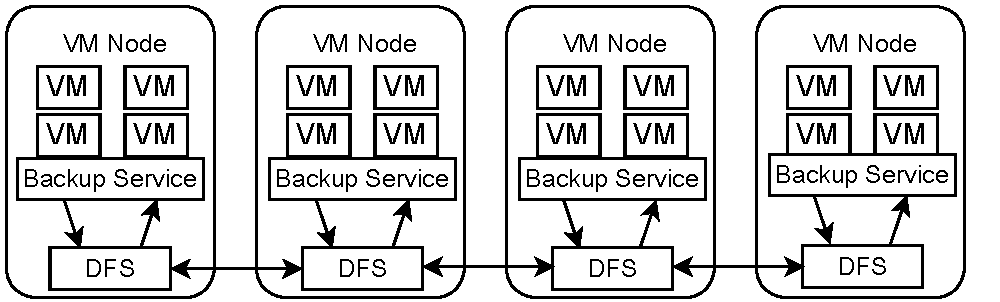
\includegraphics[width=3in]{images/colocated-arch}
    \caption{Collocated VM Backup System.}
    \label{fig:collocated}
\end{figure}

%{\em Collocating with cluster-based cloud services.}
%We collocate the backup service with other cloud services in a cluster
%and use a distributed file system
%store the backup with multiple replicas. 
%There might be a concern that storing many versions of snapshots would
%go against the purpose of deduplication.

%Assume on the average the compression
%ratio is $c$:1.  When the number of versions
%saved in the backup storage is $l$  on the average, 
%the amount of storage space in the cluster allocated  for the backup would be $\frac{l}{l+c}$.
%For example, when $l=5$ and $c=10$, 33\% of the cluster storage is used for the backup.
%When $l=9$ and $c=13$, storage usage is 40\%. 
%That is acceptable given today's cheap cost for disk storage.
%In the case of Alibaba, each machine hosts 25 VMs on the average and each VM uses 40GB data.
%Each machine however can typically provide over 10TB storage.
%Thus the normal disk usage  is about 1TB per machine, and adding 30\% to 100\% 
%extra space for the backup is not a practical concern, especially with the
%added benefits of cheaper running costs and lower network bandwidth requirements.

We discuss the design considerations as follows. 
\begin{itemize}
\item {\em Deduplication localization, sharing minimization, and fault tolerance.}

%Previous work in deduplication~\cite{extreme_binning09,sparseindex09} has
%studied the solutions to reduce memory requirements.
%One important issue not considered in the previous work is how 
Because a data chunk is compared with signatures collected from other VMs during
the deduplication process, only one copy of duplicates is stored in the backup storage
and this artificially creates data dependency among different VM users. 
Content sharing via deduplication affects fault isolation since machine failures happen at daily 
basis in a large-scale cloud and
%failure of a shared block affects many VMs.
%the loss of a shared chunks can affect many VM users whose snapshots share this 
%data block. 
loss of a small number of shared data chunks can 
cause the unavailability of snapshots for a large number of virtual machines.
Localizing the impact of deduplication can increase fault isolation and resilience.
Thus from the fault tolerance point of view,  duplicate sharing among multiple VMs is 
discourage. 
Another disadvantage of sharing is that it complicates snapshot deletion.
The mark-sweep approach~\cite{mark-sweep} is effective for deletion, and its main cost
is to count if a data chunk is still shared by other snapshots.
Thus our goal is to localize deduplication and minimize sharing, while we seek for 
a tradeoff since there are a significant number of duplicates cross VMs.
 
% since storage for shared identical content chunks can become a failure point.
%Without any control of such data sharing, we can only increase  
%replication for global datasets to enhance the availability,
%but this incurs significantly higher costs.
%Thus a key goal  in our design
%is restricting the impact of  data loss to a limited number of VMs. 
%It is not desirable that small scale of data failure affects the backup of many VMs.
%when users access snapshots in a recovery process. 
\item{\bf Packaging  data chunks as file system blocks.}
Since the file block size in the Hadoop and GFS is uniform and large with 64MB as a default setting,
the content chunk in a deduplication system is of nonuniform size with 4KB or 8KB on average.
We need to build an intermediate layer that supports large snapshot writing with append operations
and infrequent snapshot access.
Packaging that maps data chunks to file system blocks can create data dependence among VMs
since a file block can be shared even more VMs.
Thus we need to consider a minimum association of a fie system block to VMs in the packaging process.
%The distributed file system~\cite{GoogleFS,Hadoop} provides the replication support
%and we can leverage existing open-source software to implement such a layer.
%When the number of machines failed exceeds the replication degree, there could be
% some data loss.  
%Storage deduplication worsens the impact of such faults
%because  the majority of each snapshot (e.g. over 90\%) is deduplicated
%and the corresponding data chunks stored in the underlying file blocks
%are shared by many VMs. 
%The failure of one data chunk or block can impact many sharing VMs. 
\end{itemize}

%\item {\em Requirement for backup throughput and low computing resource usage}.
Because of collocation of this snapshot service with other existing cloud services, 
%As a large-scale cluster hosting tens of thousand of active VMs everyday,  the amount of data
%to be processed can be huge. 
cloud providers wish that the backup service only consumes  small resources
with a minimal impact to the existing cloud services.
%the computing resources allocated for the snapshot service is limited, especially
%because of its lower priority.
The key usage of resource for backup is memory for storing and comparing the fingerprints. 
We will consider the approximation techniques with less memory consumption
studied in~\cite{extreme_binning09,Guo2011} along with the fault isolation consideration discussed below. 
%A snapshot backup service shall not compete cpu, memory, or I/O bandwidth with VMs. 
%Fingerprint-based search does require a significant amount of memory for fingerprint lookup
%and comparison.  This competes memory resource  with the existing VMs.
%Our design is to identify a low-cost and low-profile scheme for deduplication.
%Specifically, the memory usage of snapshot service can never exceed 500MB in any node.
%Excessive use of bandwidth and computing resource for backup can create
%noticeable contention for resources with the existing cloud, which is not
%preferred and may not not be acceptable for production system operation. 
%Thus it is desirable that backup for all nodes
%can be conducted in parallel and in a short period of time,
%and any centralized or cross-machine communication for
%deduplication should not become a bottleneck.
%For example, in an Aliyun cluster with over 1,000 nodes and each hosts over 25 VMs, 
%the system must finish saving daily snapshots of all VMs in a few hours. 
%Often a cloud has a few hours of light workload each day (e.g. midnight),  
%which creates an small window for automatic backup.
%The backup service can generate hundreds of terabytes of data in such a time window
%without optimization and thus the resource content is considered carefully as we design
%a fault-resilient cluster-based solution. 
%In our typical 1000 nodes cluster, each node hosts 25 VMs, each VM has 40GB of data on average, that translates to backup throughput of 139GB/second, or 
%500TB/hour.  The system must finish saving daily snapshots of all VMs in few hours. 

%At Aliyun, it is required that while CPU and disk usage should be small or modest during backup time,
%the memory footprint of snapshot service should not exceed 500MB at each node.


\comments{
Another consideration is backup data cleaning to delete useless blocks.
Keeping reference counters for shared data blocks is challenging and less reliable.
The previous work has advocated the mark-and-sweep approach  which periodically
scans all data (or modified latest version of data)~\cite{?, Guo2011}. It first marks
all used blocks and then sweep all chunks to reclaim unmarked blocks. 
This approach is resilient to errors: at any time the process can simply be restarted with no 
negative side effects.  Scalability, however, is an issue.
To deal with 1 PB snapshots data, which may be represented by 10,000 GB FP index,
If we account for an average deduplication factor of 10 (i.e., each chunk
is referenced by 10 different snapshots), the total size
of snapshot metadata that need to be read during the mark phase will
be 100 TB.  This alone will take almost 2 hours on a
1000-machine cloud. Furthermore, marking the in-use
bits for 250 billion entries is no easy task. There is no
way to put the bit map in memory. One might want
to mitigate the poor performance of mark-and-sweep by
doing it less frequently. But in practice this is not a viable
option: customers always want to keep the utilization
of the system close to its capacity so that a longer
history can be stored. With daily snapshots taking place,
systems rarely have the luxury to postpone deletion operations
for a long time. In our field deployment, deletion
is done once a day. More than 2 hours in each run is too
much. In a large production-oriented deduplication system reference
management needs to be very reliable and have
good recover-ability. It should tolerate errors and always
ensure correctness. Although mark-and-sweep provides
these properties, its performance is proportional to the
capacity of the system, thus limiting its scalability.

}



%we want to isolate 
%each VM's snapshot backup as much as possible while still enjoy the benefit of deduplication.
%In large scale cloud, node faiures happen at daily basis, we don't want a problem at small scale
%to affect large amount of VMs due to data sharing.
%a key weakness of global content fingerprint comparison is that it affects fault isolation.

%2) data sharing among users for accessing common signagutes causes the system less resilient to storage failures.
%any loss of one piece of  shared data content hash and actualcontent will damange many VM snapshots, which can cause massive impacts
%on reliability of many users.

%Another point is that the previous work in signature-based comparison does not address
%load balancing for a distributed environment during parallel access.  
%Some content signatures can be extremely hot, but the machines  that  handle such signatures can become
% a bottleneck. Uncoordinated signature assignment could lead to imbalanced access workload.


%There are multiple choices of snapshot backup design for VM images and our considerations are described
%as follows. 
%Our design considerations
%\begin{enumerate}
%\item {\bf Centralized vs. decenalized} 
%
%It is desirable to have  a decentralized architecture.
%Given a large amount of snapshot data communicated from each machine to the backup storage,
%with a distributed storage architecture for backup, one could exploit  exploit data locality between
%the source of data and storage location of data to reduce cross-platform bandwidth requirement for backup.

%execute in parallel and easy to coordinate. In fact, we want to avoid cross-node dependency at scheduling VM snapshot operations, such that no global coordinator is necessary.
%\item {Load balancing in resource consumption}: the cost of snapshot service shall be evenly distributed onto every node. We don't have a super powerful
%or stable node that can accept extra responsibility.
%\item {minimization of inter-user data dependency for fault tolerance}: we want to minimize the data dependency to a controllable level. Data deduplication means sharing of data, thus one failure at a single point may affect the snapshot service of hundreds of VMs, which is absolutely unacceptable.
%\item {Resource usage modeling and control}.
%\end{enumerate}


A deduplication scheme compares the fingerprints of the current snapshot
with its parent snapshot and also other snapshots in the entire cloud without consideration of .
%The traditional approach compares all fingerprints and
%stores one copy for all of a chunk's duplicates.
We call this as  the VM-oblivious (VO) approach.
In designing and selecting a duplication algorithm, we have considered the following options.
\begin{itemize}
\item {\bf Version-based change detection}.
VM snapshots can be  backed up  incrementally by identifying file  blocks that have
changed from the previous version of the snapshot~\cite{Clements2009,Vrable2009,TanIPDPS2011}.
Active snapshots will contain all the information needed to restore the virtual disk
and when deleting a snapshot, data referenced by other snapshots are removed.
While full signature comparison can deliver additional reduction~\cite{Guo2011,Dong,ExtremeBining},
content change detection falls into a VM-centric approach since deduplication is localizable. 
We are seeking for additional optimization to improve duplication efficiency and design the 
association of data chunks with the underlying file blocks so that
file block sharing among VMs is minimized.
\item {\bf sampled Index}.
One alternative approach to reducing the use of memory space is 
to use a sampled index with prefetching, proposed  by Guo and Efstathopoulos\cite{Guo2011}. 
An evaluation with our test data shows that using a sampled index can achieve a high
deduplication efficiency with a single machine setup.  
One key problem is that the algorithm is VM oblivious and not easy to be adopted for VM-centric.
Another problem is  to design a distributed version 
in deduplicating large bodies of data. 
%The algorithm stores the sampled index in memory, which is required for high
%throughput to avoid the disk-bottleneck problem - since the index itself has no
%locality information, lookups are essentially random, so the index must be
%somehow optimized to prevent excessive disk seeking (the sampling algorithm does
%this by storing the index in memory). 
To use a distributed memory version of the sampled index, every deduplicate request
may access a remote machine for index lookup,  which  incurs a significant overhead.


Another possibility is to use this approach partially  in our VM centric solution by indexing
the most popular data chunks. For a small set of popular data chunks, the prefetching strategy
used in the sampled index will not work well because the spatial locality is limited among popular 
data chunks. In our test data,  on average the number of consecutive data chunks is 7, which is too small
to be effective for index sampling. 

%To distribute this sampled index, every  each machine would
%either require a complete copy of the index which would have a prohibitive cost in
%memory, or something like memcached must be used, which leaves the same problem
%as the disk bottleneck with every index check potentially using the network.
%The difficulty in storing extremely large bodies of data
%is related, as once 1PB is stored in the system, assuming a sampling rate of 
%1/101 with 22 byte index entires, 55GB of (in memory) index are required.

%Our solution uses more total memory (??how much??), but is more scalable both in
%terms of capactity and distributing the deduplication. The only part of our
%algorithm which requires significant network traffic is the PDS deduplication,
%but this is done after Levels 1 and 2 (dirty bits and comparison to parent), and
%so is only done for a small percent of blocks (?? 5-10\% ??).

\item {\bf Stateless  Data Routing}.
Another approach for duplicate comparison  is to use a content-based hash
partitioning algorithm called stateless data routing~\cite{Dong20??}
that divides the deduplication work with an approximation, which 
is similar to Exreme Binning\cite{extreme_binning09}. 
Again such an approach is VM-oblivious while each request does incur a network routing latency, and then
additional overhead for a bloomer filter based  disk lookup~\cite{Dong20??} or 
a disk index access~\cite{extreme_binning09}. 
 
%We compared our solution to
%content-based hash partitioning by running the algorithm on our set of 
%traces. We used 2MB superchunks and 4KB chunks to partition the data, and use
%the minhashes of the superchunks for routing. The results of this are shown in
%Table~\ref{??}. Routing each chunk to a bin provides good deduplication
%efficiency, and only requires each storage node to keep an index of local data
%and the bin mapping, but misses significant opportunities in our indended use
%case.

%The problem with the Data Routing algorithm is in the very high network traffic.
%Our intended use case is a backup system which runs alongside a number of VMs,
%in order to save costs. Data Routing makes no use of the inherent locality in
%such a system, and therefore puts a much higher network burden on machines which
%are also running 35 VMs each. This will reduce the available network bandwidth
%to users of the VMs, and/or reduce the possible deduplication throughput.
\end{itemize}

With these considerations in mind, we study a 
VM-centric approach (called VC)
for a backup service co-hosted   in the existing set of machines and resource usage is friendly
to the existing applications.  
We will first discuss and analyze the integration of the VM-centric deduplication strategies with fault isolation, and then present
an architecture and implementation design with deletion support.

%The deduplication process is first conducted among snapshots within each VM
%and then is conducted across VMs.  
%Given the concern that searching duplicates across VMs is a global feature which can affect parallel performance
%and complicate failure management,
%we only eliminate the duplication of a small but popular data set while still maintaining a cost-effective deduplication ratio.
%For this purpose, we exploit the data characteristics of snapshots and collect most popular data.
%Data sharing across VMs is limited within this small data set such that adding replicas for it could enhance fault tolerance.
%
%in the  our studies show that there are a large amount of data unmodified in VM snapshots
%and shared among many users (e.g. OS data). The sharing pattern follows a zip-like distribution.
%With this characteristic, we can store a small amount of popular data items which coverage a large amount of
%snapshot data blocks. 
%We discuss our design and data analysis in the next section.


%This method is based on the observation of two facts in Aliyun's VM cloud: first, VM's OS disks contain 
%huge amount of operating system and software related data which is almost never modified during VM's life span. 
%Second, the duplication pattern of user generated data follows Zipf-like law, thus a tiny set of hottest data
%take up the majority of data duplication. As a result, if we extract these hot data as a common data set,
%then most of data duplication will emerge by searching in this very small scope.


%For example, In cloud storage, we are solving data deduplication problem in a different context of 
%data stream deduplication (the D2D case): our snapshot storage service is co-located with runtime VMs,
%thus we have very limited amount of system resource leave for data deduplication. For example,
%in Aliyun's 8-core, 48GB memory, 12TB VM server, there lives over 20 VMs who are hungrily competing for
%system resources: some may running map-reduce jobs, some may serving busy web requests, 
%some may storing backend databases, any behavior that affects user VMs performance or stability is unacceptable.

%To reduce the cost of deduplication, we must confine the scope of searching duplicates as much as possible,
%thus some hints are needed to tell us where the most likely duplicates would hide. 
%Several form of hints have been used in the past: many D2D systems exploits locality,
%which bases on the fact that duplicates are likely to appear in the same sequence as they have arrived before.
%Similarity is another popular hint, it suggests that two sets of data blocks may contain lots of
%duplicates if they are indetified as similar by certain similarity detection measurements.



%\section{Architecture design and Deduplication for Snapshot Support}
%
%\section{Popularity analysis}
% data on what data popular.
%
%Analysis: modeling: singular
%
%Compute: Cache hit ratio vs. cache cost (memory cost).


\comments{
\section{Challenges}
\subsection{Indexing}
Most deduplication systems operate at the sub-file level:
a file or a data stream is divided into a sequence of fixed
or variable sized segments. For each segment, a cryptographic
hash (MD5, SHA-1/2, etc.) is calculated as its
fingerprint (FP), and it is used to uniquely identify that
particular segment. A fingerprint index is used as a catalog
of fingerprints stored in the system, allowing the detection
of duplicates: during backup, if a tuple of the form <
FP, location > exists in the index for a particular
FP, then a reference to the existing copy of the chunk
is created. Otherwise, the chunk is considered new, a
copy is stored on the server and the index is updated accordingly.
In many systems, the FP index is also crucial
for the restore process, as index entries are used to locate
the exact storage location of the chunks the backup
consists of.

The index needs to have three important properties:
1) scale to high capacities, 2) achieve good indexing
throughput, and 3) provide high duplicate detection
rate—i.e., high deduplication efficiency. Table 1 demonstrates
how these goals become very challenging for a
Petascale system. Consider a typical virtualized cloud 
in which 10,000 VMs store 1 PB data, and the
chunk size is 4 KB (for fine-granularity duplicate detection),
indexing capacity will need to be at least 10,000
GB to support all 250 billion objects in the system. Such
an index is impossible to maintain in memory. Storing it
on disk, however, would greatly reduce query throughput.
To support 1000 concurrent snapshot backup tasks, 
an aggregate throughput of 20 GB/sec, would require the
index and the whole deduplication system for that matter
to provide a query service throughput of at least 5,000
Kops/sec. Trying to scale to 1 PB by storing the index
on disk would make it impossible to achieve this level
of performance. Making the chunk size larger (e.g.,
128 KB) would make deduplication far more coarse and
severely reduce its efficiency.

Even we can distribute the index over the cloud machines,
the resources that can be allocated to system services are
limited to minimize the negative impact to user experiences. 
So it becomes obvious that efficient, scalable indexing is
a hard problem. On top of all other indexing challenges,
one must point out that chunk FPs are cryptographic
hashes, randomly distributed in the index. Adjacent index
entries share no locality and any kind of simple readahead
scheme could not amortize the cost of storing index
entries on disk.


\subsection{Deletion}
Contrary to a traditional backup system, a dedupe system
shares data among files by default. 
Since snapshots in VM cloud face constant deletion, 
reference management
is necessary to keep track of chunk usage and reclaim
freed space. In addition to scalability and speed, reliability
is another challenge for reference management.
If a chunk gets freed while it is still referenced by snapshots,
data loss occurs and files cannot be restored. On the other
hand, if a chunk is referenced when it is actually no
longer in use, it causes storage leakage.

For simplicity, many previous works only investigated simple reference
counting without considering reliability
and recoverability. Reference counting, however, suffers
from low reliability, since it is vulnerable to lost or repeated
updates: when errors occur some chunks may
be updated and some may not. Complicated transaction
rollback logic is required to make reference counts consistent.
Moreover, if a chunk becomes corrupted, it is
important to know which files are using it so as to recover
the lost segment by backing up the file again. Unfortunately,
reference counting cannot provide such information.
Finally, there is almost no way to verify if the
reference count is correct or not in a large dynamic system.
Our field feedback indicates that power outages and
data corruption are really not that rare. In real deployments,
where data integrity and recoverability directly
affect product reputation, simple reference counting is
unsatisfactory.

Maintaining a reference list is a better solution: it is
immune to repeated updates and it can identify the files
that use a particular segment. However, some kind of logging
is still necessary to ensure correctness in the case of
lost operations. More importantly, variable length reference
lists need to be stored on disk for each chunk.
Every time a reference list is updated, the whole list (and
possibly its adjacent reference lists—due to the lists’
variable length) must be rewritten. This greatly hurts the
speed of reference management.

Mark-and-sweep is generally a better solution. 
During the mark phase, all snapshot metadata are traversed 
so as to mark the used chunks. 
In the sweep phase all chunks are swept and unmarked chunks are reclaimed. 
This approach is very resilient to errors: 
at any time the process can simply be restarted with no negative side effects. 
Scalability, however, is an issue.
To deal with 1 PB snapshots data, which may be represented by 10,000 GB FP index,
If we account
for an average deduplication factor of 10 (i.e., each chunk
is referenced by 10 different snapshots),
the total size
of snapshot metadata that need to be read during the mark phase will
be 100 TB. 
This alone will take almost 2 hours on a
1000-machine cloud. Furthermore, marking the in-use
bits for 250 billion entries is no easy task. There is no
way to put the bit map in memory. One might want
to mitigate the poor performance of mark-and-sweep by
doing it less frequently. But in practice this is not a viable
option: customers always want to keep the utilization
of the system close to its capacity so that a longer
history can be stored. With daily snapshots taking place,
systems rarely have the luxury to postpone deletion operations
for a long time. In our field deployment, deletion
is done once a day. More than 2 hours in each run is too
much. In a large production-oriented dedupe system reference
management needs to be very reliable and have
good recoverability. It should tolerate errors and always
ensure correctness. Although mark-and-sweep provides
these properties, its performance is proportional to the
capacity of the system, thus limiting its scalability.

\subsection{Fault Tolerance}
Because deduplication storage system
 artificially creates data dependency among different VM users,
it increases the risk of data availability.
In large scale cloud, node failures happen at daily basis,
the loss of access to a shared chunk can affect many VMs whose snapshots share this chunk. 
Without any control of the scope of data sharing, we can only increase the level of 
replication to enhance availability, which would significantly 
balance out the benefits of deduplication.

}

\section{Prototype Design}

The architecture of our snapshot backup service contains the following components:
\begin{itemize}

\item  The backup storage layer. 
That stores snapshots on a distribued file system. 
Our prototype implementtion uses the QFS.
Since the distributed file system such as Hadoop and GFS takes the large block size such as 64MB,
and the data blcok size for dueduplication is nonuniform with 4KB on average,
we have added a layer to accmulate  data blocks from the deduplicated stream, and 
package them as 64MB, and apply data compression when applicable.

\item The deduplication layer.

\end{itemize}

Our architecture is built on the Aliyun platform which provides the largest public VM cloud in China. 
A typical VM cluster in our cloud environment
consists of from hundreds to thousands of physical machines, each of which can
host tens of xen-based\cite{Barham2003} VMs.

Aliyun has built a hadoop-like platform, which includes
several highly scalable cloud infrastructure services to support
 runing large scale VM cloud service:
\begin{itemize}
\item \textbf{DFS}: a distributed file system that is optimized for many large and sequential reads or appends.
%\item \textbf{KV}: a distributed key-value store for managing structured data.
\item \textbf{MapReduce}: a distributed data processing framework supports Map-Reduce\cite{Dean2004}.
\item \textbf{MemCache}: a distributed memory object caching system.
\end{itemize}
Our snapshot system and the virtual machine management service rely on these basic cloud services
to be functional:
DFS holds the responsibility of managing physical disk storage
in the cloud, all data needed for VM services, such as virtual disk images used by runtime VMs,
and snapshot data for backup purposes, reside in this distributed file system. 
In addition, our snapshot system 
places the index of CDS in MemCache for deduplication, 
and uses MapReduce to facilitate the offline
data processing. All the above services can easily find their open-source counterparts,
which shows the generality of our architecture and deduplication scheme.

User control VMs through the virtual machine management service.
During VM creation, a user chooses a pre-configured VM image or
a snapshot that contains an OS,
then the VM management service 
copies the corresponding VM image to her VM as the OS disk.
Data disks can be created and mounted onto the VM in the same way,
either empty or from an existing snapshot. 
All these virtual disks are represented as virtual disk image files in our
underline runtime VM storage system.  
To avoid network latency and congestion, 
our distributed file system place the primary replica of VM's 
image files at physical machine of VM instance.
When user deletes her VM, all the runtime virtual disk images and
their snapshot data are removed from DFS.

%ss operations
In each VM, 
the runtime I/O between virtual machine and its virtual
disks is tunneled by the virtual device driver (called TapDisk\cite{Warfield2005} at Xen).
This is also where our snapshot system is built in. Three major snapshot operations are supported:
\begin{itemize}
\item \textit{Write snapshot}: save the current state of virtual disk as a snapshot.
This is also where data deduplication would take place.
During snapshot backup, concurrent disk write is logged 
to ensure a consistent snapshot version is captured. 
\item \textit{Read snapshot}: restore the state of virtual disk from a snapshot.
\item \textit{Delete snapshot}: delete a snapshot and reclaim the disk space for unused data.
\end{itemize}

\begin{figure}[htbp]
  \centering
  %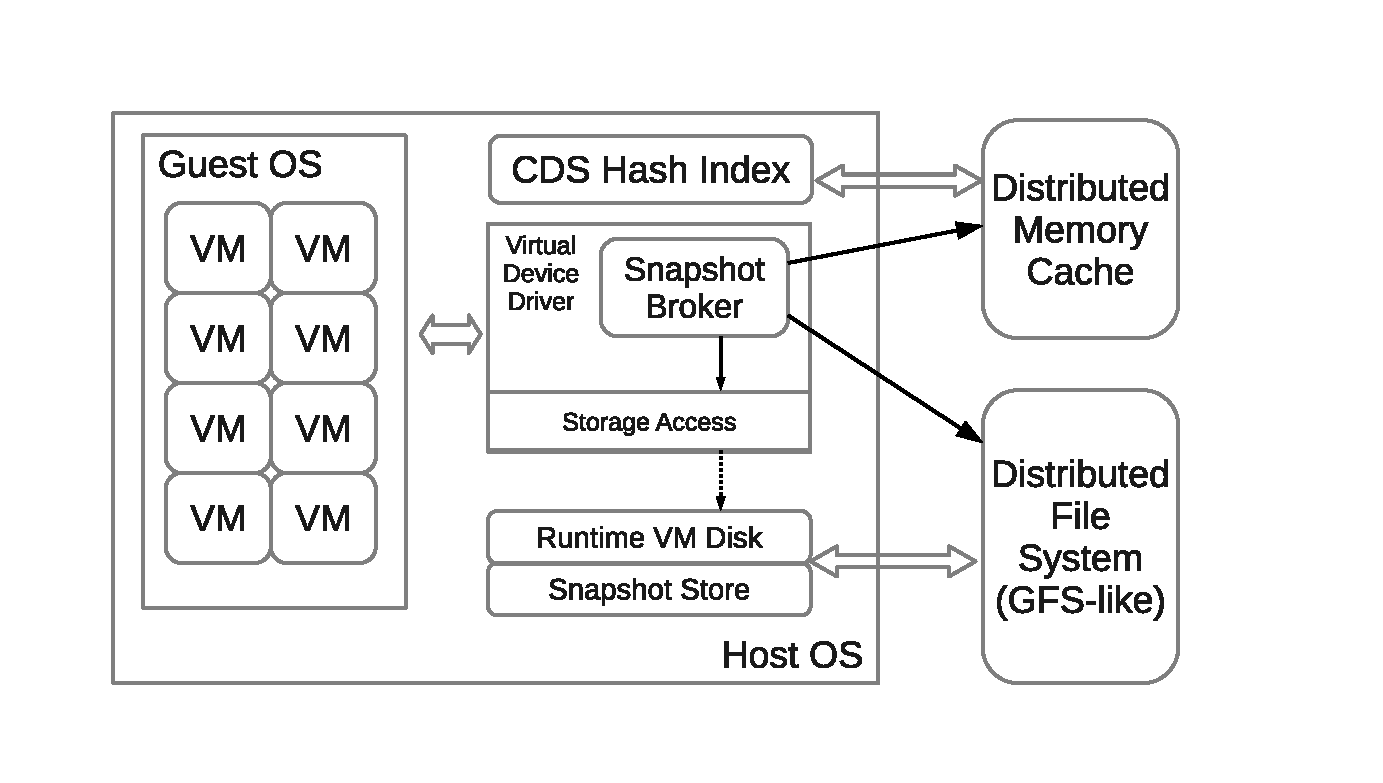
\epsfig{file=images/arch.eps, height=2in, width=2.66in}
  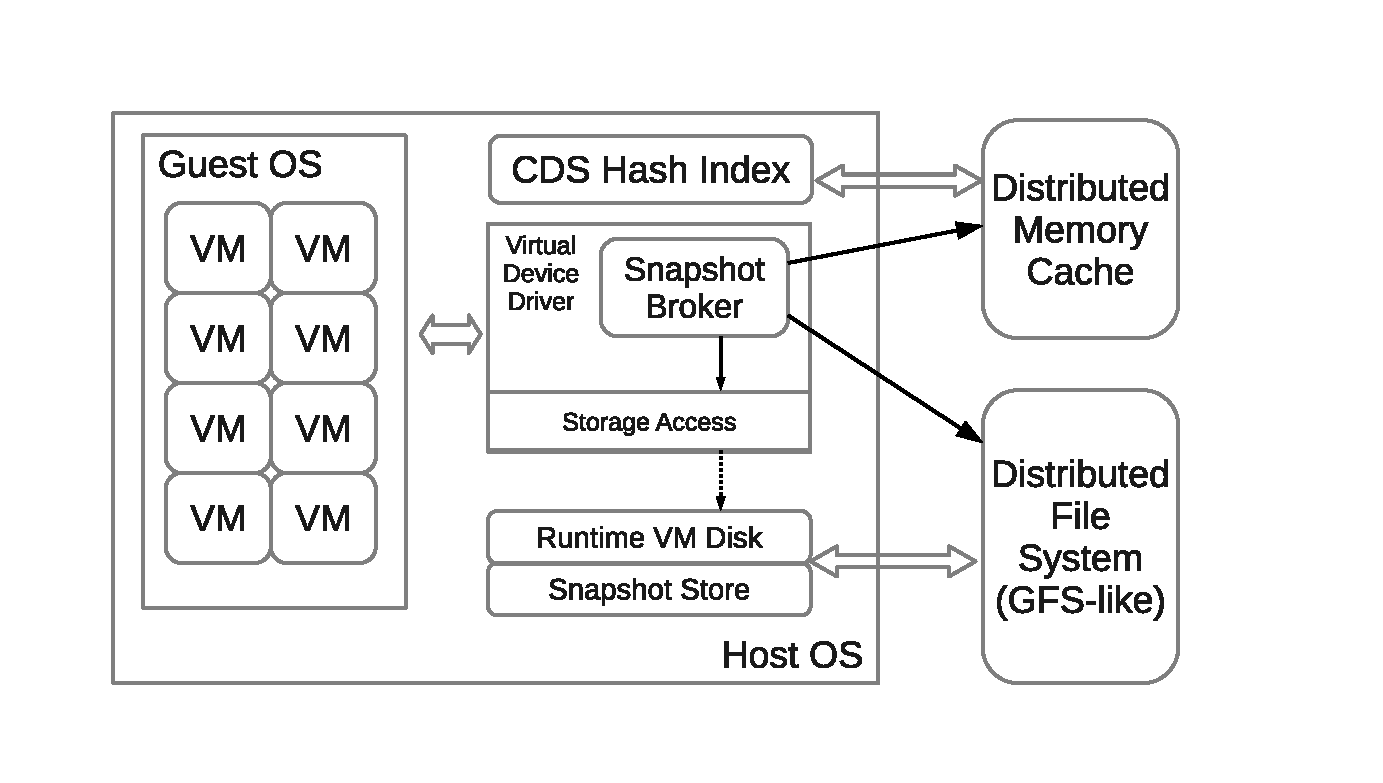
\epsfig{file=images/arch.eps, width=3.9in}
  \caption{Snapshot backup architecture of each node.}
  \label{fig:arch}
\end{figure}

Figure~\ref{fig:arch} shows the architecture view of our snapshot service
at each node. The snapshot broker provides the functional interface for  snapshot backup, access, and deletion.
The inner-VM  deduplication is conducted by the broker to access meta data in the snapshot data store
and we discuss this in details in Section~\ref{sect:innerVM}.
The cross-VM deduplication is conducted by the broker to access 
a common data set (CDS) (will discuss in Section~\ref{sect:crossVM},
whose block hash index is stored in a distributed memory cache. 

%\section{Multi-level Snapshot Deduplication}
\label{sect:dedupe}

\subsection{Snapshot System}
%system arch
Our architecture is built on the Aliyun platform which provides the largest public VM cloud in China. 
A typical VM cluster in our cloud environment
consists of from hundreds to thousands of physical machines, each of which can
host tens of xen-based\cite{Barham2003} VMs.

Aliyun has built a hadoop-like platform, which includes
several highly scalable cloud infrastructure services to support
 runing large scale VM cloud service:
\begin{itemize}
\item \textbf{DFS}: a distributed file system that is optimized for many large and sequential reads or appends.
\item \textbf{KV}: a distributed key-value store for managing structured data.
\item \textbf{MP}: a distributed data processing framework which is similar to Map-Reduce\cite{Dean2004}.
\item \textbf{MemCache}: a distributed memory object caching system.
\end{itemize}
%GFS-like\cite{googlefs03} 
%BigTable-like\cite{Chang2008a} 
Our snapshot system and the virtual machine management service rely on these basic cloud services
to be functional:
DFS holds the responsibility of managing physical disk storage
in the cloud, all data needed for VM services, such as virtual disk images used by runtime VMs,
and snapshot data for backup purposes, reside in this distributed file system. 
In addition, our snapshot system 
places the index of CDS in MemCache for deduplication, 
stores small amount of snapshot metadata in KV, and uses FX to facilitate the offline
data processing. All the above services can easily find their open-source counterparts,
which shows the generality of our architecture and deduplication scheme.

User control VMs through the virtual machine management service.
During VM creation, a user chooses a pre-configured VM image or
a snapshot that contains an OS,
then the VM management service 
copies the corresponding VM image to her VM as the OS disk.
Data disks can be created and mounted onto the VM in the same way,
either empty or from an existing snapshot. 
All these virtual disks are represented as virtual disk image files in our
underline runtime VM storage system.  
To avoid network latency and congestion, 
our distributed file system place the primary replica of VM's 
image files at physical machine of VM instance.
When user deletes her VM, all the runtime virtual disk images and
their snapshot data are removed from DFS.

%ss operations
In each VM, 
the runtime I/O between virtual machine and its virtual
disks is tunneled by the virtual device driver (called TapDisk\cite{Warfield2005} at Xen).
This is also where our snapshot system is built in. Three major snapshot operations are supported:
\begin{itemize}
\item \textit{Write snapshot}: save the current state of virtual disk as a snapshot.
This is also where data deduplication would take place.
During snapshot backup, concurrent disk write is logged 
to ensure a consistent snapshot version is captured. 
\item \textit{Read snapshot}: restore the state of virtual disk from a snapshot.
\item \textit{Delete snapshot}: delete a snapshot and reclaim the disk space for unused data.
\end{itemize}

\begin{figure}[htbp]
  \centering
  %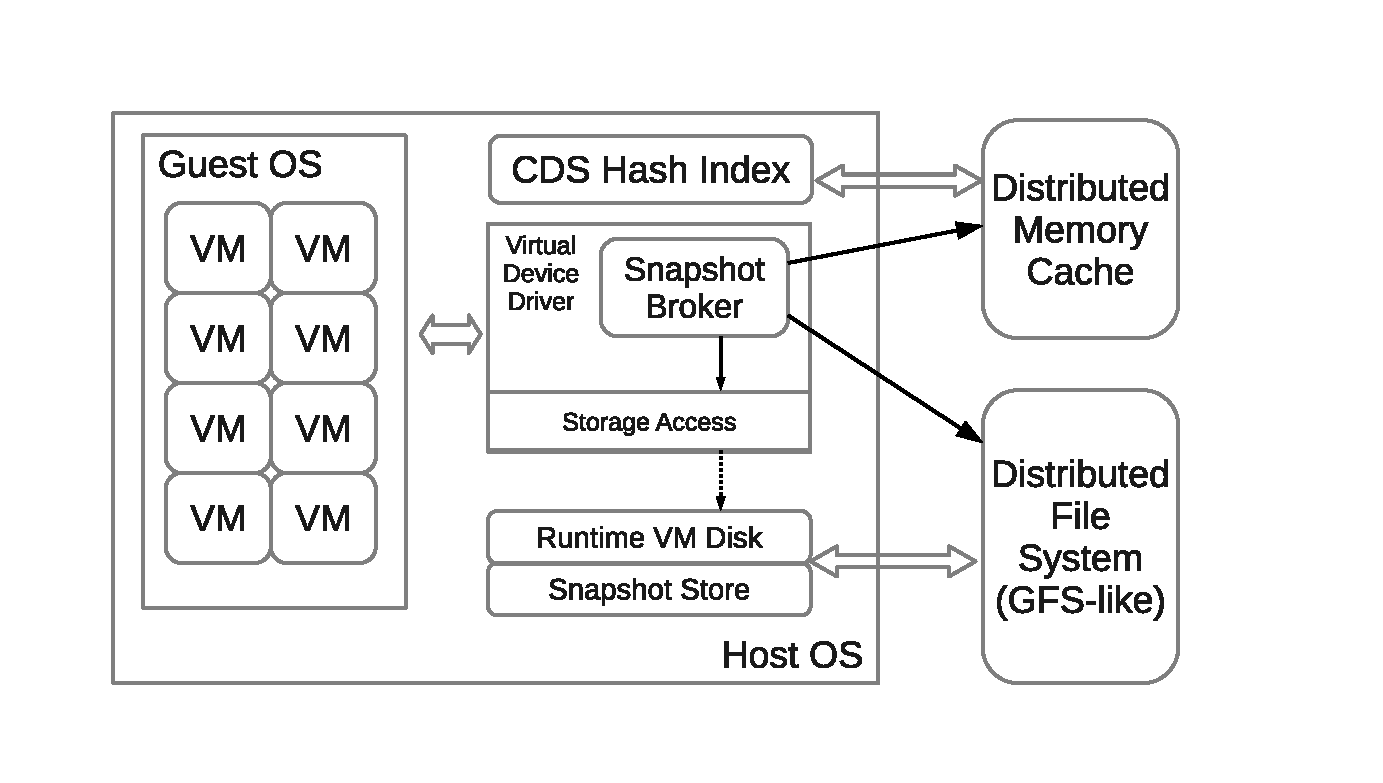
\epsfig{file=images/arch.eps, height=2in, width=2.66in}
  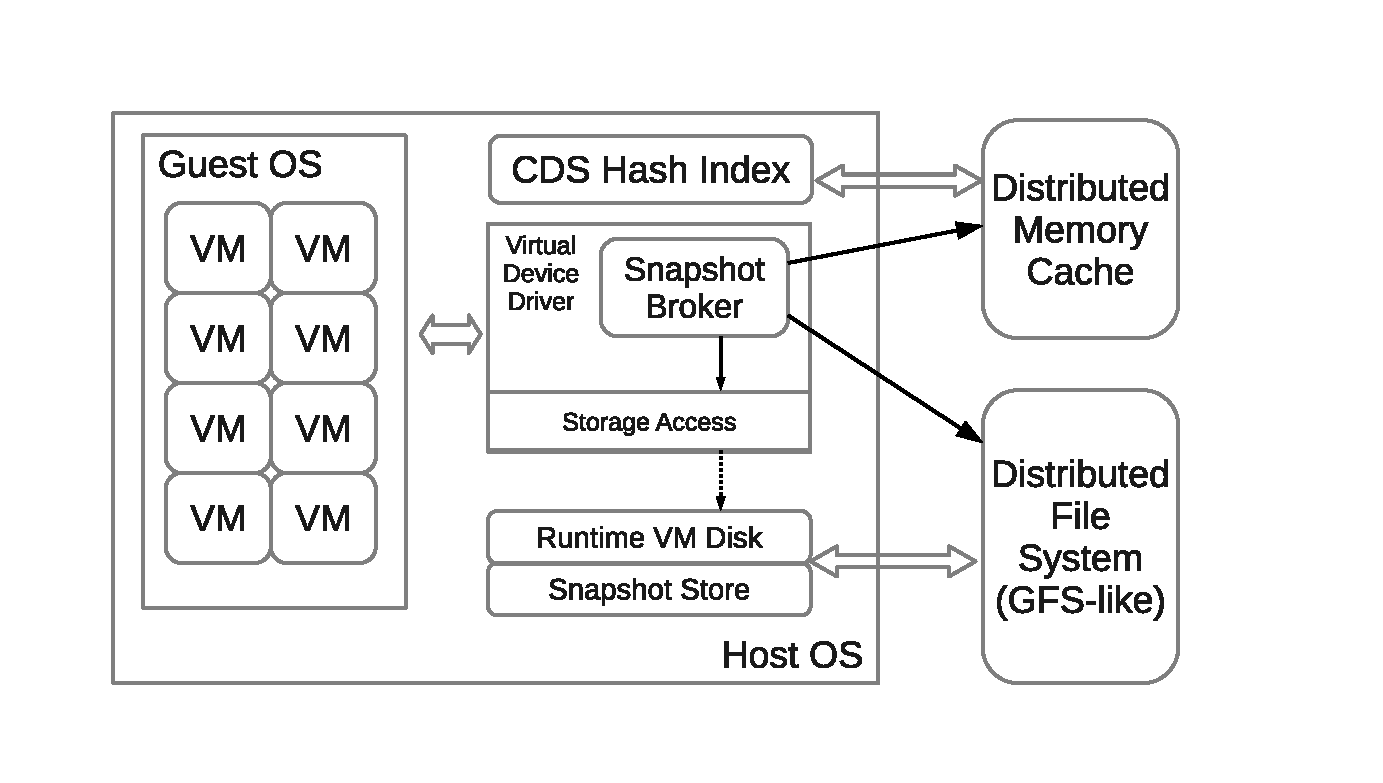
\epsfig{file=images/arch.eps, width=3.9in}
  \caption{Snapshot backup architecture of each node.}
  \label{fig:arch}
\end{figure}

Figure~\ref{fig:arch} shows the architecture view of our snapshot service
at each node. The snapshot broker provides the functional interface for  snapshot backup, access, and deletion.
The inner-VM  deduplication is conducted by the broker to access meta data in the snapshot data store
and we discuss this in details in Section~\ref{sect:innerVM}.
The cross-VM deduplication is conducted by the broker to access 
a common data set (CDS) (will discuss in Section~\ref{sect:crossVM},
whose block hash index is stored in a distributed memory cache. 

%snapshot representation
\subsection{Snapshot Representation}
The virtual device driver uses a bitmap to track the changes 
that have been made to virtual disk.
Every bit in the bitmap represents a fix-sized (2MB) region called \textit{segment}, indicates whether the segment
is modified since last backup. Hence we could treat segment as the basic unit in snapshot backup similar to
file in normal backup: a snapshot could share a segment with previous snapshot it is not changed. 
Moreover, we break 
segments into var-sized chunks (average 4KB) using content-based chunking algorithm,
which brings the opportunity of fine-grained deduplication by
allowing data sharing between segments.

\begin{figure}[htbp]
  \centering
  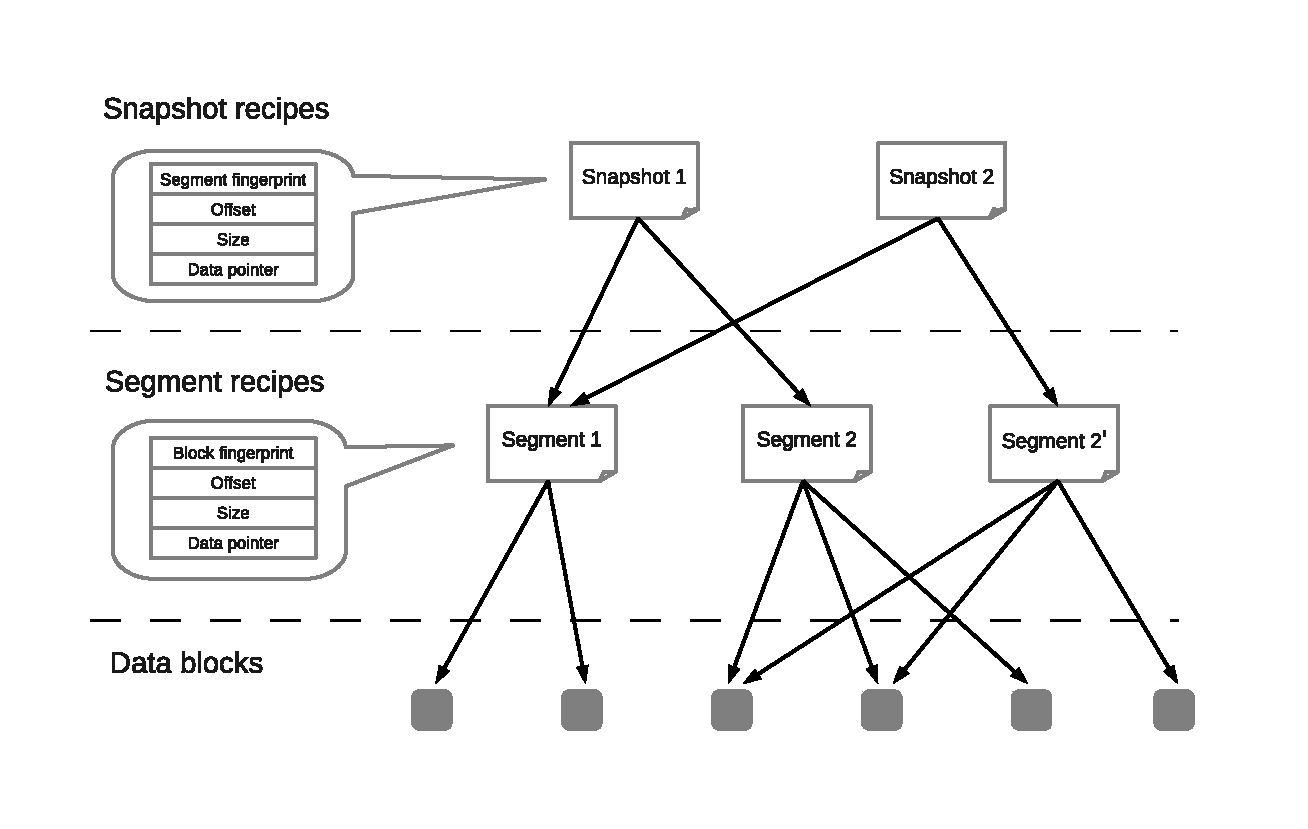
\epsfig{file=images/snapshot_representation.eps, width=3.7in}
  \caption{An example of snapshot representation.}
  \label{fig:snapshot}
\end{figure}
As a result, the representation of each snapshot is designed as a two-level index data structure 
in the form of a hierarchical directed acyclic graph as shown in Figure \ref{fig:snapshot}.
A snapshot recipe contains a list of segments, each of which is represented as a segment recipe
that holds the meatdata of its chunks. We choose this two-level structure because in practice we
observe that during each backup period only a small amount of VM data are added or modified. 
As the result, even the metadata of two snapshots can be highly similar, 
thus aggregating a large number of chunks as one segment can significantly reduce the space cost of snapshot metadata.
Furthermore, instead of using variables-sized segments, we use a dirty bit to capture the change status of fix-sized
segments which greatly ease the segment-level deduplication.

In both two kind of recipes, 
they do not include the actual data but only have
 references point to the data which are either stored in append store or CDS.
In our implementation the data reference is a 8 bytes field which is either an 
ASID (discuss in \ref{sect:append} or an offset of 
An additional flag indicates

\subsection{Multi-level Deduplication}
The multi-level deduplication scheme is designed base on the observations on the VM snapshot data from production cloud.
We found snapshot data duplication can be easily classified into two categories: \textit{Inner-VM} and \textit{Cross-VM}. 
Inner-VM duplication exists between VM's snapshots, because the majority of data are unchanged during each backup period. 
On the other hand, Cross-VM duplication is mainly due to widely-used software and libraries such as Linux and MySQL. 
As the result, different VMs tend to backup large amount of highly similar data.
Our multi-level pipeline process can minimize the cost of deduplication while maximize the its efficiency at each level,
and it is highly parallelizable since each segment is processed independently.

\subsubsection{Inner-VM Deduplication}
\label{sect:InnerVM}
The first-level deduplication is logically localized within each VM.
Such localization increases data independency between different VM backups,
simplifies snapshot management and statistics collection,
and facilitates parallel execution of snapshot operations.

The inner VM deduplication contains two levels of duplicate detection efforts:
\begin{itemize}
\item \textit{Level 1 Segment modification detection}.
If a segment is not changed, then its segment recipe can be simply reused by copying the data
reference from previous snapshot recipe. 
\item \textit{Level 2  Chunk fingerprint comparison.}
If a segment is modified, we perform fine-grained deduplication 
by comparing the fingerprints of its chunks to the same segment's recipe in the previous snapshot,
thus eliminate partial data duplication within the segment.
\end{itemize}

In general, operations at level 1 have almost no cost and most of unmodified data are filtered here. 
To process a dirty segment at level 2, 
there requires no more than one DFS access to load the segment recipe from previous snapshot,
and a tiny amount of memory to hold it in main memory.
\textit{may need details here}

\subsubsection{Cross-VM Deduplication}
\label{sect:CrossVM}

\subsection{Common Data Set}
%arch
%analysis
\section{Append Store}
\label{sect:append}
\subsection{Introduction}
Append Store (AS) is our underlining storage engine for storing snapshot data after deduplication. 
AS is built on top of our highly scalable distributed file system (DFS), 
which is very similar to Google's file system
in a sense that it is optimized for large files and sequential read/append operations.

\subsection{Design considerations}
While scalability has been handled by the DFS, there are still several challenges in 
storing billions of var-sized small data chunks:
\begin{description}
\item[Locality perseveration] Chunk data must be placed next to each other in the order of their writing sequence,
because reading a snapshot incurs large sequential reads of chunks under their logical sequence in the snapshot.
\item[Flexible referencing] To avoid overwhelming metadata operation capbility of DFS's master, 
we have to group small chunks into large data files in DFS.
However, snapshot deletion brings chunk data deletion, and reclaiming disk space would require many chunk data being moved.
If such chunk movement incurs updates of data referencing in snapshot and segment recipes, then the cost of deleting 
a snapshot would be extremely high.
\item[Efficient chunk lookup] The translation from data reference to data location must be very efficient in two ways: 
first, a sorted index is necessary to fast locate the data location in $O(log(n)$ time; 
second, the size of index must be optimized to minimized its memory footprint and the cost of fetching index. 
\end{description}



\subsection{Architecture}
\begin{figure}[htbp]
  \centering
  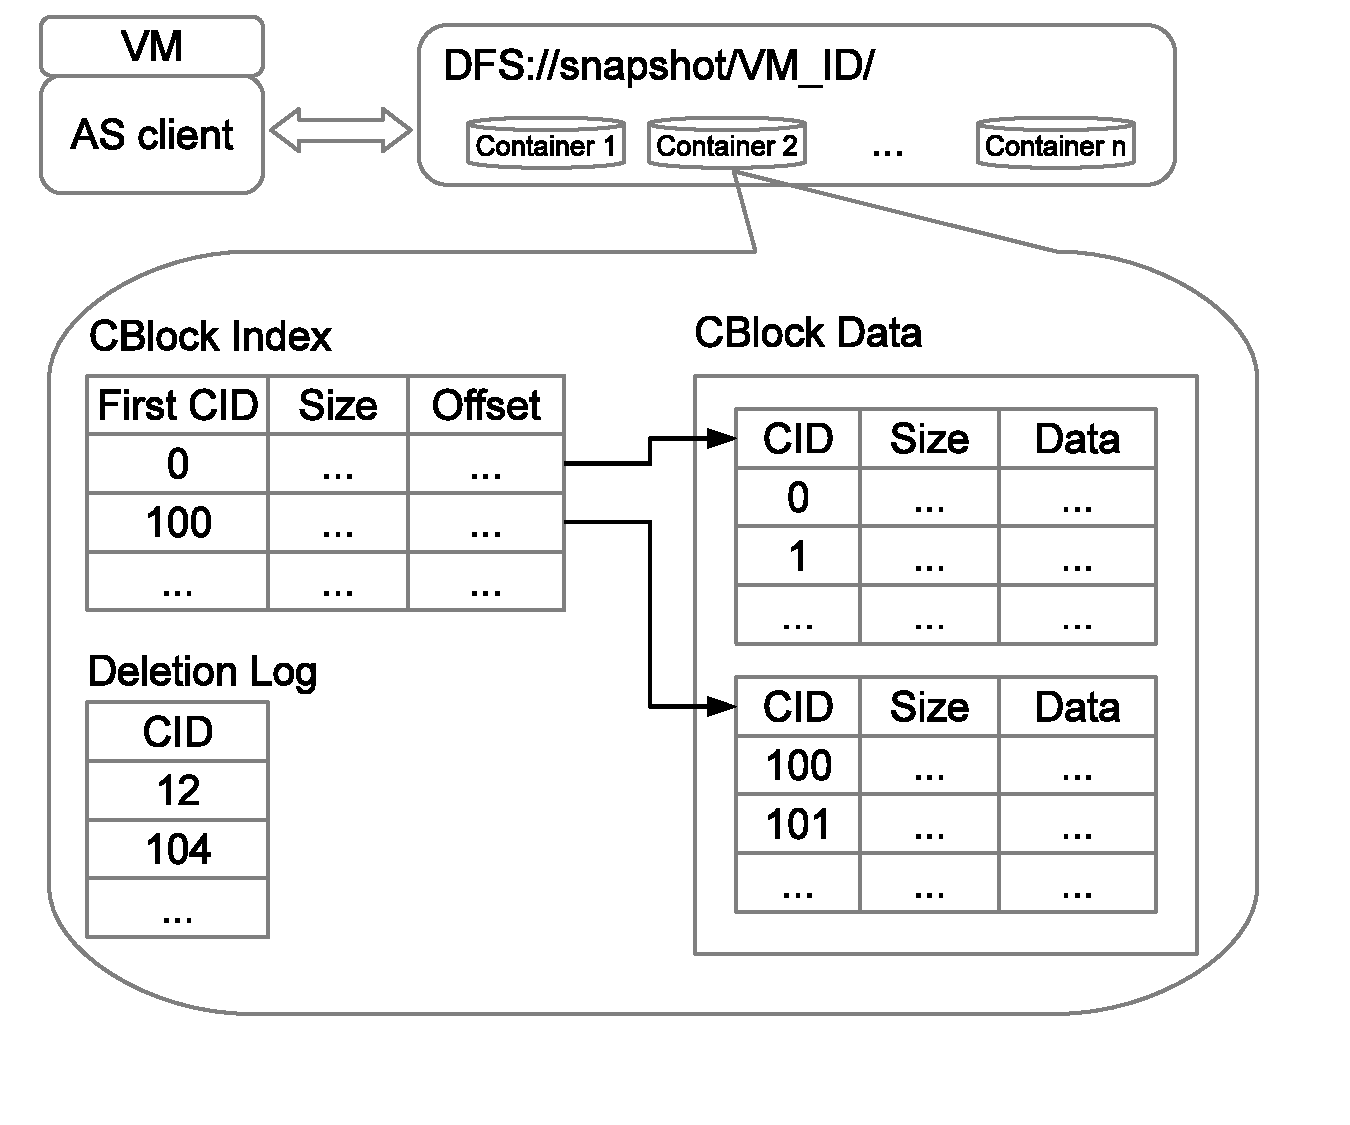
\epsfig{file=images/append_store_arch.pdf, width=3.5in}
  \caption{Architecture of Append Store}
  \label{fig:as_arch}
\end{figure}

Append Store supplies three interfaces: {\em get(ref)} accepts a data reference and retrives data, 
{\em put(data)} accepts data and returns a reference to be stored in metadata recipes, 
{\em delete(ref)} 
deletes the data pointed by the reference.
Under the hood, small var-sized data are grouped and stored into larger data containers. Each VM has
its snapshot data stored in its own Append Store, specified by the VM ID. 
We split every Append Store into multiple data containers so that reclaiming the disk space would not 
result in rewriting all the data at the same time.

As shown in Fig.\ref{fig:as_arch}, every data container is represented as three data files in DFS:
the data file holds all the actual data, the index file is responsible for translating data reference
into data locations, and a deletion log file remembers all the deletion requests to the container.

A data reference is composed of two parts: a container ID (2 bytes) and CID (6 bytes).
Append Store assign every piece of data a CID for its internal data referencing. 
When new data is appended, its CID is the current largest CID in that container plus one.
As a result, all the data locations are naturally indexed by this self-incremental CID, 
no extra sorting is needed.

Append Store groups multiple chunk data (i.e., 100) into larger units, called {\em CBlock}.
CBlock is the basic unit for append store's internal read/write/compression.
There is one index entry in the container index corresponding to every CBlock. It keeps the first chunk's CID
in that CBlock, and the CBlock data's size and location.

Using CBlock brings us several advantages: First, the write workload to DFS master is greatly reduced; second, grouping
small chunks gives better compression. Third, reading a CBlock (200 - 600 KB) typically cost the same amount of disk 
seek as reading a 4KB chunk. Finally, this greatly reduces the size of index. Let $m$ be the number of chunks in each
CBlock, then the overall index size is reduced to $1/m$. In our implementation, using $m=100$ reduces the index for
a 1GB container from 10 MB to 100 KB.

\subsection{Operations}
In order to read a chunk data by reference, Append Store client first loads the
container index file specified by the container ID, then search the CBlock index to find the entry that covers the chunk by CID.
After that, it reads the whole CBlock data from DFS, decompress it, seek the exact chunk data specified by CID. 
Finally, the client updates itws internal chunk data cache with the newly loaded contents to anticipate future sequential reads.

Write requests to append store are accumlated. When the number reaches $m$, the AS client forms a CBlock by assigning 
every chunk a CID, compress the CBlock data, and append it to the CBlock data file. Then a new CBlock index entry is appended
to CBlock index.

Append store adopts lazy delete strategy. The deletion requests are appended into every container's deletion log file with the CID of data to be deleted.
CIDs in deletion log are guaranteed to be referenced by nobody and can be safe deleted in future. 
Periodically, snapshot management system asks append store to compact containers in order to reclaim disk space. 
The actual compaction will only take place when the number of deleted items reached $d\%$ of container's capacity. 
During compaction, append store creates a new container (with the same container ID) to replace the 
existing one. This is done by sequentially scan the old container, copying all the chunks that are not 
found in deletion log to the new container, creating new CBlocks and indices. 
However, every chunk's CID is plainly copied rather than re-generated. This does not affect the sorted
order of CIDs in new container, but just leaving holes in CID values. As the result, all data references stored 
in upper level recipes are unaffected, and the data reading process is as efficient as before.

%hard problems

\subsection{Analysis}

Snapshot operation performance analysis:
\begin{table}
    \begin{tabular}{l p{1.5in} l}
        \hline
        Symbol & Description & Measurement \\ \hline
        $N_{seg}$ & Number of segments in the snapshot & ~ \\ [1ex] \\ [-1.5ex]
        $N_{chunk}$ & Number of chunks in one segment & ~ \\ [1ex] \\ [-1.5ex]
        $P_{dirty}$ & Probablity of a segment is dirty & ~ \\ [1ex] \\ [-1.5ex]
        $P_{new}$ & Percentage of new data & ~ \\ [1ex] \\ [-1.5ex]
        $P_{change}$ & Probablity that a chunk is not found in parent snapshot & ~ \\ [1ex] \\ [-1.5ex]
        $P_{in\_CDS}$ & Percentage of chunks in CDS & ~ \\ [1ex] \\ [-1.5ex]
        $T_{scan}$ & Time to scan segment data and caculate content hash & 74 ms \\ [1ex] \\ [-1.5ex]
        $T_{write\_AS}$ & Time of writing a chunk into append store & 0.24 ms \\ [1ex] \\ [-1.5ex]
        $T_{read\_AS}$ & Time of reading a chunk from append store & ~ \\ [1ex] \\ [-1.5ex]
        $T_{read\_chunk}$ & Time of reading a chunk & ~ \\ [1ex] \\ [-1.5ex]
        $T_{check\_CDS}$ & Time of checking CDS & ~ \\ [1ex] \\ [-1.5ex]
        $T_{read\_CDS}$ & Time of reading a chunk data from CDS data store& ~ \\
        \hline
    \end{tabular}
    \caption{List of performance factors}
    \label{tab:as_param}
\end{table}

The overall time of writing a snapshot is:

\begin{dmath}
T_{write} = P_{dirty} * N_{seg} * [max(T_{scan}, T_{read\_AS}) + P_{change} * N_{chunk} * T_{check\_CDS} + P_{new} * N_{chunk} * T_{write\_AS}]
\end{dmath}

The overall time to read a snapshot is:

\begin{dmath}
T_{read} = N_{seg} * {T_{read\_AS} + N_{chunks} * [P_{in\_CDS} * T_{read_CDS} + (1 - P_{in\_CDS}) * T_{read\_chunk}]}
\end{dmath}

Average time of reading a chunk:

\begin{dmath}
T_{read\_chunk} = P_{in\_CDS} * T_{read\_CDS} + (1 - P_{in\_CDS}) * T_{read\_AS}
\end{dmath}

Time of reading append store:

\begin{dmath}
T_{read\_AS} = 0 * P_{in\_cache} + (1 - P_{in\_cache} ) * T_{load\_CBlock}
\end{dmath}

\section{Deletion}
In a mature VM cluster, snapshot deletions are as frequent as snapshot creations.
Our system adopts lazy delete strategy so that all snapshot deletions are scheduled
in the backup time window at midnight. 
Therefore, snapshot deletions must be fast enough to fit in time window and
efficient enough to satisfy our resource constraints.
However, there is no simple solution can achieve these goals with high reliability.
In Aliyun's cloud, we use a {\em fuzzy deletion} method to trade deletion accuracy for
speed and resource usage. This method tolerates a tiny percentage of storage leakage
to make the deletion operation faster and efficient by an order of magnitude,
yet we still adopt an slow but accurate deletion method to fix such leakage in the long-term.
Our hybrid deletion strategy, using fuzzy deletion regularly and accurate deletion periodically,
accomplishs our speed, resource usage and relibility goals very well.

% \subsection{Challenges}
% Contrary to a traditional backup system, a dedupe system shares data among files by default. 
% Reference management is necessary to keep track of chunk usage and reclaim freed space. 
% In addition to scalability and speed, reliability is another challenge for reference management. 
% If a chunk gets freed while it is still referenced by snapshots, data loss occurs and files cannot be restored. 
% On the other hand, if a chunk is referenced when it is actually no longer in use, it causes storage leakage.

% Reference counting, while being simple, suffers from low reliability especially in our distributed environment, 
% because it is vulnerable to lost or repeated updates: when errors occur some chunks maybe updated and some may not. 
% Complicated transaction rollback logic is required to make reference counts consistent. Moreover, 
% there is almost no way to verify if the reference count is correct or not in a large dynamic system. 
% In real deployments, where data integrity and recoverability directly affect product reputation, simple reference counting is unsatisfactory.

% Mark-and-sweep is generally a better solution. During the mark phase, all snapshot recipes are traversed so as to mark the used chunks. 
% In the sweep phase all chunks are swept and unmarked chunks are reclaimed. 
% This approach is very resilient to errors: at any time the process can simply be restarted with no negative side effects. 
% Scalability, however, is an issue. {\em needs to explain its resource usage}


\subsection{Approximate Deletion}
\begin{figure}[htbp]
  \centering
  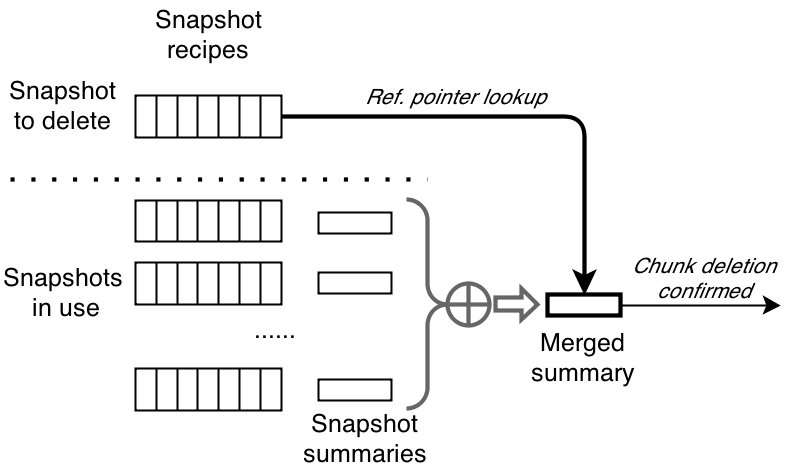
\epsfig{file=images/deletion.png, width=3.5in}
  \caption{Approximate deletion}
  \label{fig:deletion_flow}
\end{figure}

We design approximate deletion to fast identify unused data in the append store.
Instead of scanning the whold append store, it uses a bloom filter to check 
if a data are still referenced by living snapshots. However, there is a small false-positive probility which
would indetify unused data as in use, i.e., storage leakage.
The following steps would take place during an approximate deletion:

\begin{enumerate}
\item {\bf Creating bloom filter} Scan all the living snapshot recipess and their segment recipes,
for every reference pointing to append store, add it to the bloom filter.
\item {\bf Check existance} For every data reference in the deleted snapshot recipe and its segment recipes,
check the existance of that data reference in bloom filter. If not found, it is safe to delete that piece of data from append store
because no living snapshots has referenced it.
\end{enumerate}

The overall time of running a approximate deletion for one snapshot deletion would be scanning
all the living snapshots and deleted snapshots, since operations on the in-memory bloom filter can be done in
parallel and is much faster than loading recipes from DFS:
\begin{equation}
T = (N_{SS} + 1) * T_{scan\_recipes}
\end{equation}
 
Using the example and analysis in previous section, this approximate deletion can be done in 5 minutes. 
Memory usage of the bloom filter depends on its false-positive probility $P_{bl}$,
when set $P_{bl}$ to 0.01, the memory footprint of approximate deletion is about 15 MB.

The design goal of approximate deletion is to reduce the frequency of running accurate deletion.
For one VM's snapshots, let $D_{leakage}$ be the amount of storage leakage, $D_{del}$ be the average amount of data
to be deleted in one snapshot deletion, 
then we have:
\begin{equation}
D_{leakage} = N_{approximate} * P_{bl} * D_{del}
\end{equation}
where $N_{approximate}$ is the number of runs of approximate deletion. 
An accurate deletion is triggered to fix the storage leakage
when $D_{leakage}/D_{del}$ is accmulated to exceed certain threshold $T$:
\begin{equation}
D_{leakage} / D_{del} = N_{approximate} * P_{bl} > T \Rightarrow N_{approximate} > T/P_{bl}
\end{equation}
Therefore, when $P_{bl} = 0.01$ and $T=1$, 
there would be a run of accurate deletion for every $T/P_{bl} = 100$ runs of approximate deletion.
On a machine that hosts 20 VMs and each VM deletes snapshot daily, there would be less than
one accurate deletion scheduled per day.

\subsection{Accurate Deletion}
Our accurate deletion uses mark-and-sweep to find all the unused chunks in a VM's append store.
The following steps would take place during an accurate deletion:

\begin{enumerate}
\item Scan all the containers. For each container, extract full list of existing data references and allocate a bitmap. 
(Notice this list is self sorted.)
\item Scan all the snapshot recipes and segment recipes. For every data reference pointing to append store,
find it in the above lists and mark the corresponding position in bitmaps.
\item Scan the bitmaps, for every bit that are not marked, tell append store the corresponding data reference can be deleted.
\end{enumerate}

Although accurate deletion guarantees reliability and correctness, its speed and resource usage are big problems to our VM cloud.
Let $T_{scan\_AS}$ be the time to scan the VM's append store, $T_{scan\_recipes}$ be the time to scan one snapshot recipe
and its segment recipes, $T_{mark}$ be the time of finding a data reference in the list and mark bitmap, 
$N_{SS}$ be the number of snapshots and $N_c$ be the number of chunks in one snapshot.
The overall time of running an accurate deletion for one VM is:
\begin{equation}
T = T_{scan\_AS} + N_{SS} * T_{scan\_recipes} + N_{SS} * N_c * T_{mark}
\end{equation}

For a virtual disk that has 10 snapshots, 50 GB of data in the append store, $T_{scan\_AS}$ would have cost half an hour already.
In addition, scanning recipes of 10 snapshots cost another 5 minutes.
Furthermore, maintaining the full lists of data references and bitmaps costs about 100 MB of memory. Having tens of VMs
co-lived in one physical machine and deleting snapshot on a daily basis, 
it's infeasible to run accurate deletion as frequent as snapshot deletions.

\subsection{Discussion}


%\section{Multi-level Snapshot Deduplication}
\label{sect:dedupe}

\subsection{Snapshot System}
%system arch
Our architecture is built on the Aliyun platform which provides the largest public VM cloud in China. 
A typical VM cluster in our cloud environment
consists of from hundreds to thousands of physical machines, each of which can
host tens of xen-based\cite{Barham2003} VMs.

Aliyun has built a hadoop-like platform, which includes
several highly scalable cloud infrastructure services to support
 runing large scale VM cloud service:
\begin{itemize}
\item \textbf{DFS}: a distributed file system that is optimized for many large and sequential reads or appends.
\item \textbf{KV}: a distributed key-value store for managing structured data.
\item \textbf{MP}: a distributed data processing framework which is similar to Map-Reduce\cite{Dean2004}.
\item \textbf{MemCache}: a distributed memory object caching system.
\end{itemize}
%GFS-like\cite{googlefs03} 
%BigTable-like\cite{Chang2008a} 
Our snapshot system and the virtual machine management service rely on these basic cloud services
to be functional:
DFS holds the responsibility of managing physical disk storage
in the cloud, all data needed for VM services, such as virtual disk images used by runtime VMs,
and snapshot data for backup purposes, reside in this distributed file system. 
In addition, our snapshot system 
places the index of CDS in MemCache for deduplication, 
stores small amount of snapshot metadata in KV, and uses FX to facilitate the offline
data processing. All the above services can easily find their open-source counterparts,
which shows the generality of our architecture and deduplication scheme.

User control VMs through the virtual machine management service.
During VM creation, a user chooses a pre-configured VM image or
a snapshot that contains an OS,
then the VM management service 
copies the corresponding VM image to her VM as the OS disk.
Data disks can be created and mounted onto the VM in the same way,
either empty or from an existing snapshot. 
All these virtual disks are represented as virtual disk image files in our
underline runtime VM storage system.  
To avoid network latency and congestion, 
our distributed file system place the primary replica of VM's 
image files at physical machine of VM instance.
When user deletes her VM, all the runtime virtual disk images and
their snapshot data are removed from DFS.

%ss operations
In each VM, 
the runtime I/O between virtual machine and its virtual
disks is tunneled by the virtual device driver (called TapDisk\cite{Warfield2005} at Xen).
This is also where our snapshot system is built in. Three major snapshot operations are supported:
\begin{itemize}
\item \textit{Write snapshot}: save the current state of virtual disk as a snapshot.
This is also where data deduplication would take place.
During snapshot backup, concurrent disk write is logged 
to ensure a consistent snapshot version is captured. 
\item \textit{Read snapshot}: restore the state of virtual disk from a snapshot.
\item \textit{Delete snapshot}: delete a snapshot and reclaim the disk space for unused data.
\end{itemize}

\begin{figure}[htbp]
  \centering
  %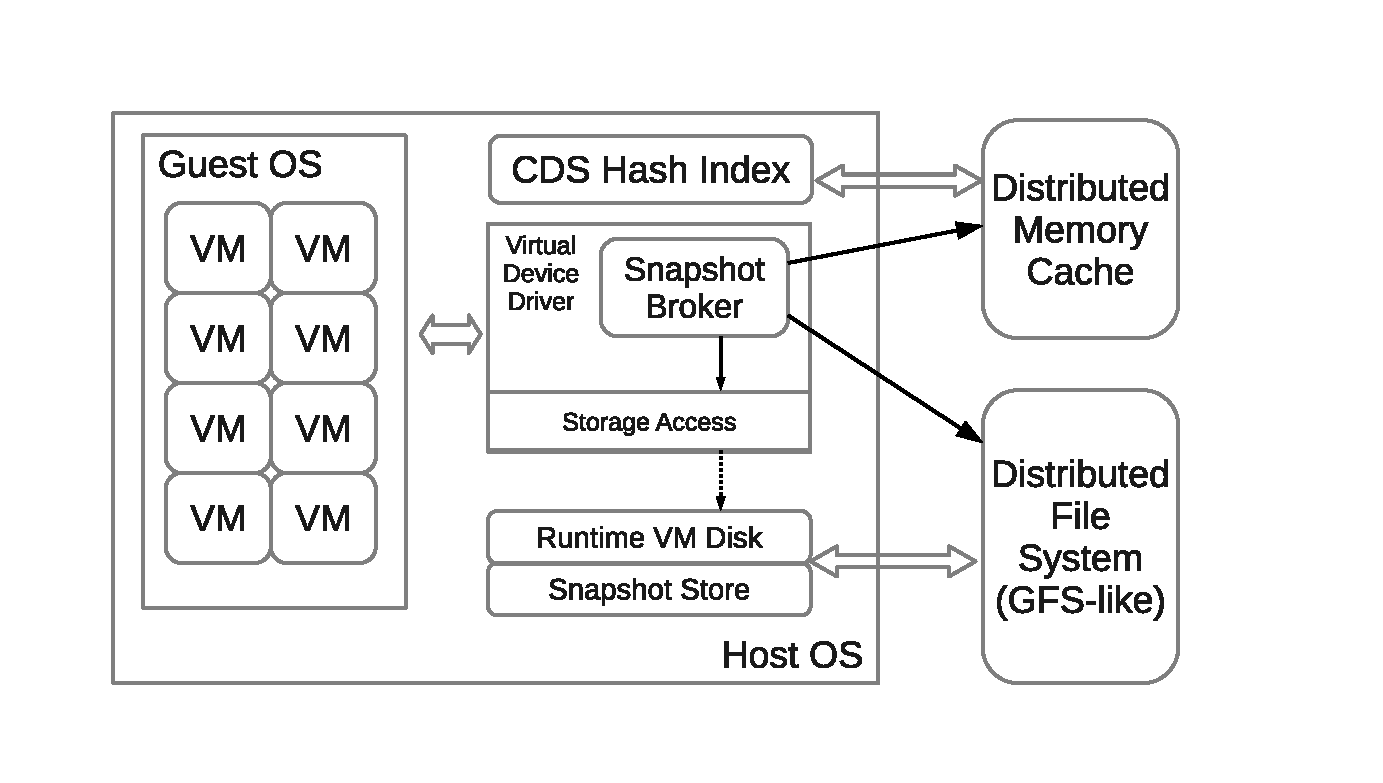
\epsfig{file=images/arch.eps, height=2in, width=2.66in}
  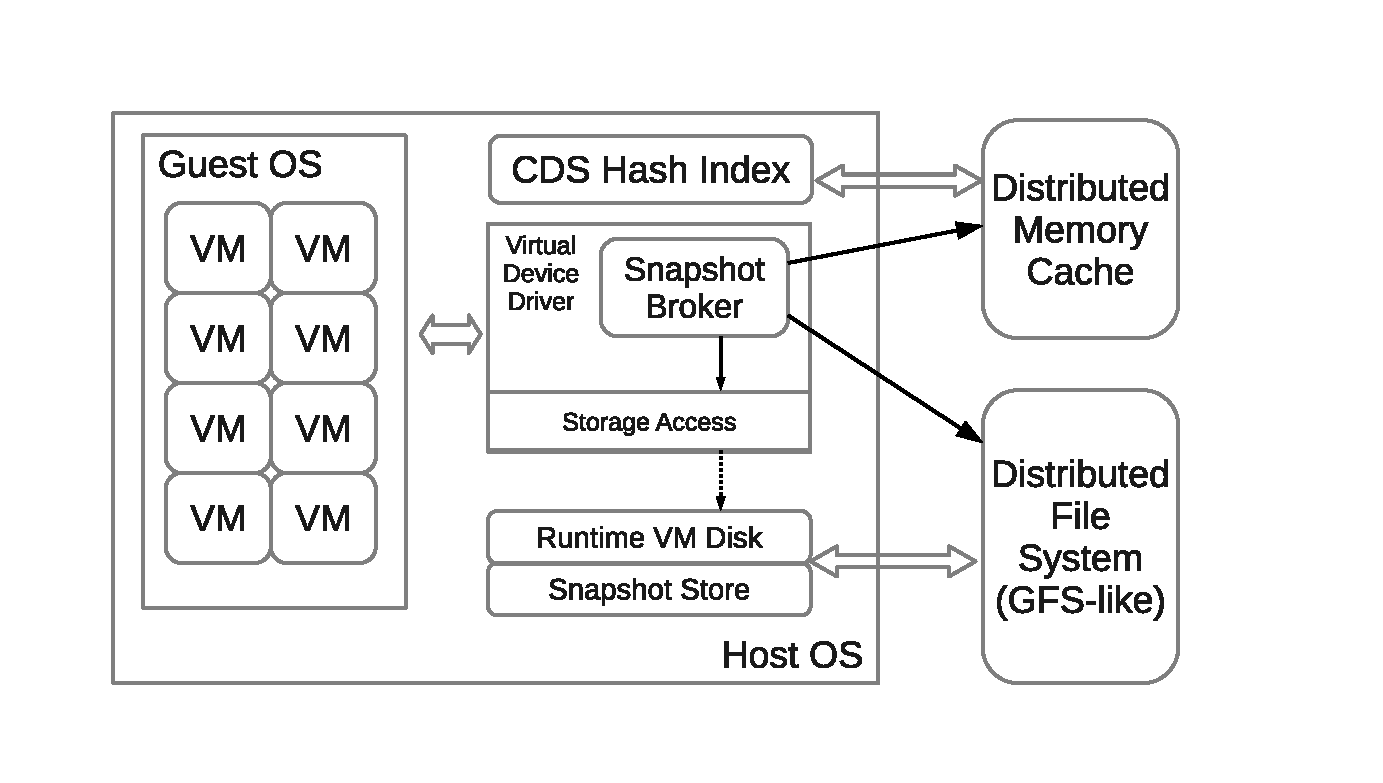
\epsfig{file=images/arch.eps, width=3.9in}
  \caption{Snapshot backup architecture of each node.}
  \label{fig:arch}
\end{figure}

Figure~\ref{fig:arch} shows the architecture view of our snapshot service
at each node. The snapshot broker provides the functional interface for  snapshot backup, access, and deletion.
The inner-VM  deduplication is conducted by the broker to access meta data in the snapshot data store
and we discuss this in details in Section~\ref{sect:innerVM}.
The cross-VM deduplication is conducted by the broker to access 
a common data set (CDS) (will discuss in Section~\ref{sect:crossVM},
whose block hash index is stored in a distributed memory cache. 

%snapshot representation
\subsection{Snapshot Representation}
The virtual device driver uses a bitmap to track the changes 
that have been made to virtual disk.
Every bit in the bitmap represents a fix-sized (2MB) region called \textit{segment}, indicates whether the segment
is modified since last backup. Hence we could treat segment as the basic unit in snapshot backup similar to
file in normal backup: a snapshot could share a segment with previous snapshot it is not changed. 
Moreover, we break 
segments into var-sized chunks (average 4KB) using content-based chunking algorithm,
which brings the opportunity of fine-grained deduplication by
allowing data sharing between segments.

\begin{figure}[htbp]
  \centering
  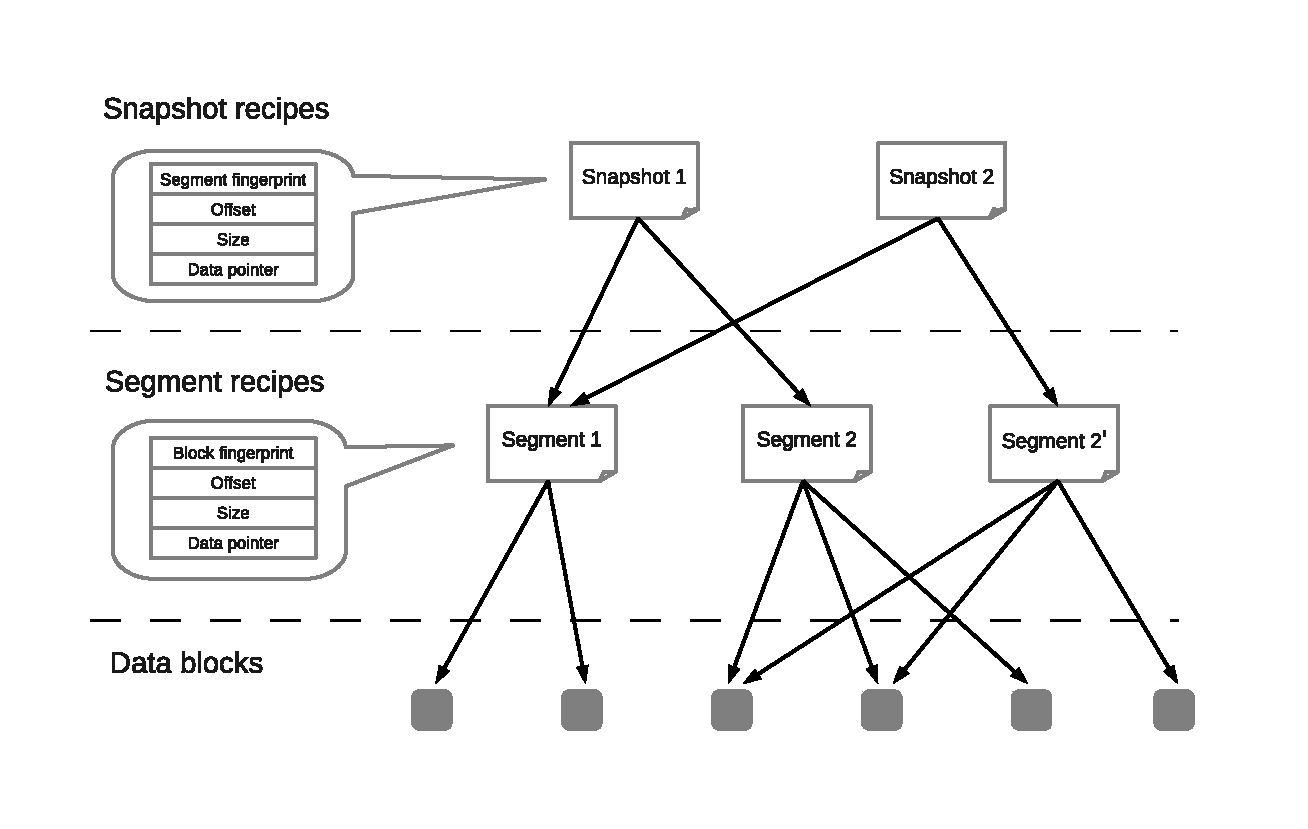
\epsfig{file=images/snapshot_representation.eps, width=3.7in}
  \caption{An example of snapshot representation.}
  \label{fig:snapshot}
\end{figure}
As a result, the representation of each snapshot is designed as a two-level index data structure 
in the form of a hierarchical directed acyclic graph as shown in Figure \ref{fig:snapshot}.
A snapshot recipe contains a list of segments, each of which is represented as a segment recipe
that holds the meatdata of its chunks. We choose this two-level structure because in practice we
observe that during each backup period only a small amount of VM data are added or modified. 
As the result, even the metadata of two snapshots can be highly similar, 
thus aggregating a large number of chunks as one segment can significantly reduce the space cost of snapshot metadata.
Furthermore, instead of using variables-sized segments, we use a dirty bit to capture the change status of fix-sized
segments which greatly ease the segment-level deduplication.

In both two kind of recipes, 
they do not include the actual data but only have
 references point to the data which are either stored in append store or CDS.
In our implementation the data reference is a 8 bytes field which is either an 
ASID (discuss in \ref{sect:append} or an offset of 
An additional flag indicates

\subsection{Multi-level Deduplication}
The multi-level deduplication scheme is designed base on the observations on the VM snapshot data from production cloud.
We found snapshot data duplication can be easily classified into two categories: \textit{Inner-VM} and \textit{Cross-VM}. 
Inner-VM duplication exists between VM's snapshots, because the majority of data are unchanged during each backup period. 
On the other hand, Cross-VM duplication is mainly due to widely-used software and libraries such as Linux and MySQL. 
As the result, different VMs tend to backup large amount of highly similar data.
Our multi-level pipeline process can minimize the cost of deduplication while maximize the its efficiency at each level,
and it is highly parallelizable since each segment is processed independently.

\subsubsection{Inner-VM Deduplication}
\label{sect:InnerVM}
The first-level deduplication is logically localized within each VM.
Such localization increases data independency between different VM backups,
simplifies snapshot management and statistics collection,
and facilitates parallel execution of snapshot operations.

The inner VM deduplication contains two levels of duplicate detection efforts:
\begin{itemize}
\item \textit{Level 1 Segment modification detection}.
If a segment is not changed, then its segment recipe can be simply reused by copying the data
reference from previous snapshot recipe. 
\item \textit{Level 2  Chunk fingerprint comparison.}
If a segment is modified, we perform fine-grained deduplication 
by comparing the fingerprints of its chunks to the same segment's recipe in the previous snapshot,
thus eliminate partial data duplication within the segment.
\end{itemize}

In general, operations at level 1 have almost no cost and most of unmodified data are filtered here. 
To process a dirty segment at level 2, 
there requires no more than one DFS access to load the segment recipe from previous snapshot,
and a tiny amount of memory to hold it in main memory.
\textit{may need details here}

\subsubsection{Cross-VM Deduplication}
\label{sect:CrossVM}

\subsection{Common Data Set}
%arch
%analysis
%\section{Append Store}
\label{sect:append}
\subsection{Introduction}
Append Store (AS) is our underlining storage engine for storing snapshot data after deduplication. 
AS is built on top of our highly scalable distributed file system (DFS), 
which is very similar to Google's file system
in a sense that it is optimized for large files and sequential read/append operations.

\subsection{Design considerations}
While scalability has been handled by the DFS, there are still several challenges in 
storing billions of var-sized small data chunks:
\begin{description}
\item[Locality perseveration] Chunk data must be placed next to each other in the order of their writing sequence,
because reading a snapshot incurs large sequential reads of chunks under their logical sequence in the snapshot.
\item[Flexible referencing] To avoid overwhelming metadata operation capbility of DFS's master, 
we have to group small chunks into large data files in DFS.
However, snapshot deletion brings chunk data deletion, and reclaiming disk space would require many chunk data being moved.
If such chunk movement incurs updates of data referencing in snapshot and segment recipes, then the cost of deleting 
a snapshot would be extremely high.
\item[Efficient chunk lookup] The translation from data reference to data location must be very efficient in two ways: 
first, a sorted index is necessary to fast locate the data location in $O(log(n)$ time; 
second, the size of index must be optimized to minimized its memory footprint and the cost of fetching index. 
\end{description}



\subsection{Architecture}
\begin{figure}[htbp]
  \centering
  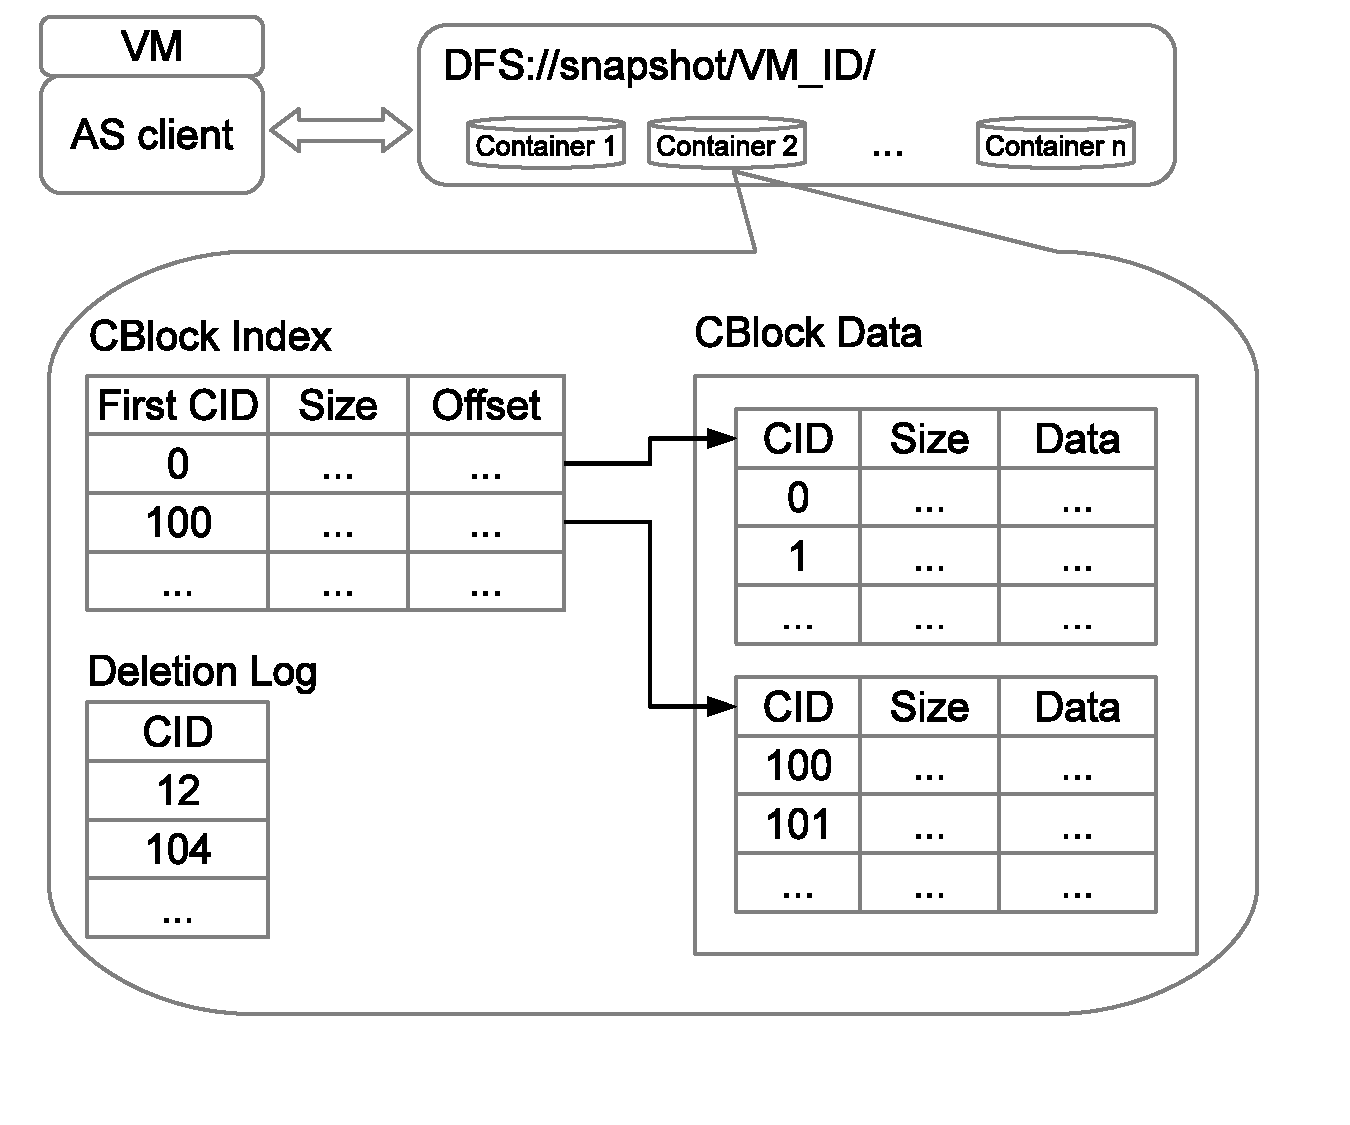
\epsfig{file=images/append_store_arch.pdf, width=3.5in}
  \caption{Architecture of Append Store}
  \label{fig:as_arch}
\end{figure}

Append Store supplies three interfaces: {\em get(ref)} accepts a data reference and retrives data, 
{\em put(data)} accepts data and returns a reference to be stored in metadata recipes, 
{\em delete(ref)} 
deletes the data pointed by the reference.
Under the hood, small var-sized data are grouped and stored into larger data containers. Each VM has
its snapshot data stored in its own Append Store, specified by the VM ID. 
We split every Append Store into multiple data containers so that reclaiming the disk space would not 
result in rewriting all the data at the same time.

As shown in Fig.\ref{fig:as_arch}, every data container is represented as three data files in DFS:
the data file holds all the actual data, the index file is responsible for translating data reference
into data locations, and a deletion log file remembers all the deletion requests to the container.

A data reference is composed of two parts: a container ID (2 bytes) and CID (6 bytes).
Append Store assign every piece of data a CID for its internal data referencing. 
When new data is appended, its CID is the current largest CID in that container plus one.
As a result, all the data locations are naturally indexed by this self-incremental CID, 
no extra sorting is needed.

Append Store groups multiple chunk data (i.e., 100) into larger units, called {\em CBlock}.
CBlock is the basic unit for append store's internal read/write/compression.
There is one index entry in the container index corresponding to every CBlock. It keeps the first chunk's CID
in that CBlock, and the CBlock data's size and location.

Using CBlock brings us several advantages: First, the write workload to DFS master is greatly reduced; second, grouping
small chunks gives better compression. Third, reading a CBlock (200 - 600 KB) typically cost the same amount of disk 
seek as reading a 4KB chunk. Finally, this greatly reduces the size of index. Let $m$ be the number of chunks in each
CBlock, then the overall index size is reduced to $1/m$. In our implementation, using $m=100$ reduces the index for
a 1GB container from 10 MB to 100 KB.

\subsection{Operations}
In order to read a chunk data by reference, Append Store client first loads the
container index file specified by the container ID, then search the CBlock index to find the entry that covers the chunk by CID.
After that, it reads the whole CBlock data from DFS, decompress it, seek the exact chunk data specified by CID. 
Finally, the client updates itws internal chunk data cache with the newly loaded contents to anticipate future sequential reads.

Write requests to append store are accumlated. When the number reaches $m$, the AS client forms a CBlock by assigning 
every chunk a CID, compress the CBlock data, and append it to the CBlock data file. Then a new CBlock index entry is appended
to CBlock index.

Append store adopts lazy delete strategy. The deletion requests are appended into every container's deletion log file with the CID of data to be deleted.
CIDs in deletion log are guaranteed to be referenced by nobody and can be safe deleted in future. 
Periodically, snapshot management system asks append store to compact containers in order to reclaim disk space. 
The actual compaction will only take place when the number of deleted items reached $d\%$ of container's capacity. 
During compaction, append store creates a new container (with the same container ID) to replace the 
existing one. This is done by sequentially scan the old container, copying all the chunks that are not 
found in deletion log to the new container, creating new CBlocks and indices. 
However, every chunk's CID is plainly copied rather than re-generated. This does not affect the sorted
order of CIDs in new container, but just leaving holes in CID values. As the result, all data references stored 
in upper level recipes are unaffected, and the data reading process is as efficient as before.

%hard problems

\subsection{Analysis}

Snapshot operation performance analysis:
\begin{table}
    \begin{tabular}{l p{1.5in} l}
        \hline
        Symbol & Description & Measurement \\ \hline
        $N_{seg}$ & Number of segments in the snapshot & ~ \\ [1ex] \\ [-1.5ex]
        $N_{chunk}$ & Number of chunks in one segment & ~ \\ [1ex] \\ [-1.5ex]
        $P_{dirty}$ & Probablity of a segment is dirty & ~ \\ [1ex] \\ [-1.5ex]
        $P_{new}$ & Percentage of new data & ~ \\ [1ex] \\ [-1.5ex]
        $P_{change}$ & Probablity that a chunk is not found in parent snapshot & ~ \\ [1ex] \\ [-1.5ex]
        $P_{in\_CDS}$ & Percentage of chunks in CDS & ~ \\ [1ex] \\ [-1.5ex]
        $T_{scan}$ & Time to scan segment data and caculate content hash & 74 ms \\ [1ex] \\ [-1.5ex]
        $T_{write\_AS}$ & Time of writing a chunk into append store & 0.24 ms \\ [1ex] \\ [-1.5ex]
        $T_{read\_AS}$ & Time of reading a chunk from append store & ~ \\ [1ex] \\ [-1.5ex]
        $T_{read\_chunk}$ & Time of reading a chunk & ~ \\ [1ex] \\ [-1.5ex]
        $T_{check\_CDS}$ & Time of checking CDS & ~ \\ [1ex] \\ [-1.5ex]
        $T_{read\_CDS}$ & Time of reading a chunk data from CDS data store& ~ \\
        \hline
    \end{tabular}
    \caption{List of performance factors}
    \label{tab:as_param}
\end{table}

The overall time of writing a snapshot is:

\begin{dmath}
T_{write} = P_{dirty} * N_{seg} * [max(T_{scan}, T_{read\_AS}) + P_{change} * N_{chunk} * T_{check\_CDS} + P_{new} * N_{chunk} * T_{write\_AS}]
\end{dmath}

The overall time to read a snapshot is:

\begin{dmath}
T_{read} = N_{seg} * {T_{read\_AS} + N_{chunks} * [P_{in\_CDS} * T_{read_CDS} + (1 - P_{in\_CDS}) * T_{read\_chunk}]}
\end{dmath}

Average time of reading a chunk:

\begin{dmath}
T_{read\_chunk} = P_{in\_CDS} * T_{read\_CDS} + (1 - P_{in\_CDS}) * T_{read\_AS}
\end{dmath}

Time of reading append store:

\begin{dmath}
T_{read\_AS} = 0 * P_{in\_cache} + (1 - P_{in\_cache} ) * T_{load\_CBlock}
\end{dmath}

%\section{CDS Analysis}
Although locality based data reduction can remove most of the inner-VM duplications,
it's not able to solve the data duplication cross VMs. Different VMs still share large amount
of common data such that their snapshot backups would have a lot of data in common.
Our observations on Aliyun's real VM user data reveals several major sources of cross-VM data duplication:
  \begin{enumerate}
  \item \emph{System-related data}: These data are generated by public third-parties, they are copied/downloaded/installed into VM disks either automatically or manually. Once installed, operations on such data are mostly read only until software updates arrive. For example, data of operating systems, some widely-used software such as Apache and MySQL, and their documations all fall into this category.
  \item \emph{User-generated data}: These data are generated by individual user's behavior, either directly or indirectly. They are much less duplicated than the system-related data, but the zipf-like distribution indicates that a small amount of data in this category could represent most of data duplications.
  \item \emph{Zero-filled data}: Like previous studies [refs here], we've observed that zero-filled data exist pervasively at system wide. They are almost like the spaces and commas in text articles. Under content-based chunking, they were distilled as zero-filled blocks with the maximum allowed length. 
%Zero-filled blocks are mostly generated by user behavior to preserve the space for future data, thus we treat them as a special case of user-generated data.
  \end{enumerate}

Without eliminating the data duplication between VM snapshot backups, storage space is severely wasted when the number of VMs increases.
To address this problem, we developed a technique called \emph{Common Data Set (CDS)} to eliminate data duplication for all three situations above. 
CDS is a public data library that shared by all VM snapshot backups in the cluster, 
which consists of the most popular data blocks in VM snapshot backups. It is generated, 
managed and accessed in an uniform manner by all VMs such that [write some fancy system characteristic stuff here].

\subsection{CDS Size V.S. Coverage}
As a shared data library, we expect CDS to collect almost all the system related data, the most popular user-generated data and the zero-filled data block.
With CDS as a public data reference, each VM's snapshot backup has no need to store its own copies for data that can be found in CDS, instead they can just
store a reference.

The more data we put into CDS, the closer we come to complete deduplication. But in reality we are facing a list of restrictions such like [blabla].
We borrowed the idea of web caching[refs here] to analysis the size of CDS vesus its effectiveness on data reduction.

We let $M$ be the number of nodes in a cluster, $N$ be the number of VMs hosted per node,
and let $D$ denotes the average size of one VM's snapshot backups (after level 1 and 2 reduction, which is near 40 GB in our production environment).
And let $C_0$, $C_s$ and $C_u$ denote the size of zero-filled block, system-related data and user-generated data in CDS,
then the total size of CDS is represented by $C=C_0+C_s+C_u$.
We let $S_0$, $S_s$ and $S_u$ denote the corresponding data coverage ratio (with respect to $D$) by $C_0$, $C_s$ and $C_u$,
so the total space saving ratio is $S=S_0+S_s+S_u$.

Zero-filled block at maximum length is the first item we need to put into CDS. This is the one and only special data block, 
and because CDS only stores unique data blocks, $C_0$ is almost equal to 0. In practice we found zero-filled blocks account
for near 20\% of total data, so $S_0$ is 20\%.

The rarely modified system-related data are the second to be added to CDS. We have thousands of VMs in each cluster, 
but all these VMs fall into only a few OS types, using a limited selection of software, therefore data duplication in this category
is highly noticable in a global block counting. In particular, most of such data already exist in the VM base images. 
We analyzed VMs running various services from 7 mainstream OS types in our cluster, and found close to 50GB of such data in total. 
Because system-related data don't change frequently, it's safe to expect that for 20 OS variations 
and software updates in 2 years, $C_s$ will not grow to exceed 200 GB.
For each VM, from 2 to 20 GB of data can be reduced in this way, depends on the OS and service type, so on average we estimate
$S_s$ would be no less than 20\%.

The rest of data are user-generated, the total size of such data can be written as $D_u=D-S_0-S_s$, which is 60\% of $D$. 
It follows a zipf-like distribution with $\alpha$ between 0.65 to 0.7. 
Let $T_u$ be the total size of unique data blocks in $D_u$,
in practice we notice that complete deduplication for such data always result in a 2:1 reduction ratio,
, so $T_u=D_u/2$.
Since we collect the most popular user-generated data into CDS, the coverage of CDS on user-generated data
is $(C_u/T_u)^{1-\alpha}$.

The following table lists CDS coverage on user-generated data under different $\alpha$ and $C_u/T_u$.

[a table of coverage with alpha from 0.65-0.70, ratio from 0.002 0.005 0.01 0.02 0.05]

It's obviously that at least 30\% of user-generated data can be reduced in this way, using about 0.02 of $T_u$, or 0.01 of $D_u$.
The size of user-generated data in CDS would be 0.006$D$, with coverage $S_u=0.18D$.

Thus the estimation of CDS coverage is $S=S_0+S_s+S_u=0.58$, with the size of CDS to be no more than $(200 + 0.006*D*N)$ GB.
In a VM cluster of 100 machines, with 25 VMs on each physical machine, the size of CDS is 800 GB in total, or 8 GB per machine.
The total size of CDS index would be 8 GB, which will cost 80 MB memory on each machine. 

\subsection{CDS Access}

\subsection{CDS Management}


%\section{Deletion}
In a mature VM cluster, snapshot deletions are as frequent as snapshot creations.
Our system adopts lazy delete strategy so that all snapshot deletions are scheduled
in the backup time window at midnight. 
Therefore, snapshot deletions must be fast enough to fit in time window and
efficient enough to satisfy our resource constraints.
However, there is no simple solution can achieve these goals with high reliability.
In Aliyun's cloud, we use a {\em fuzzy deletion} method to trade deletion accuracy for
speed and resource usage. This method tolerates a tiny percentage of storage leakage
to make the deletion operation faster and efficient by an order of magnitude,
yet we still adopt an slow but accurate deletion method to fix such leakage in the long-term.
Our hybrid deletion strategy, using fuzzy deletion regularly and accurate deletion periodically,
accomplishs our speed, resource usage and relibility goals very well.

% \subsection{Challenges}
% Contrary to a traditional backup system, a dedupe system shares data among files by default. 
% Reference management is necessary to keep track of chunk usage and reclaim freed space. 
% In addition to scalability and speed, reliability is another challenge for reference management. 
% If a chunk gets freed while it is still referenced by snapshots, data loss occurs and files cannot be restored. 
% On the other hand, if a chunk is referenced when it is actually no longer in use, it causes storage leakage.

% Reference counting, while being simple, suffers from low reliability especially in our distributed environment, 
% because it is vulnerable to lost or repeated updates: when errors occur some chunks maybe updated and some may not. 
% Complicated transaction rollback logic is required to make reference counts consistent. Moreover, 
% there is almost no way to verify if the reference count is correct or not in a large dynamic system. 
% In real deployments, where data integrity and recoverability directly affect product reputation, simple reference counting is unsatisfactory.

% Mark-and-sweep is generally a better solution. During the mark phase, all snapshot recipes are traversed so as to mark the used chunks. 
% In the sweep phase all chunks are swept and unmarked chunks are reclaimed. 
% This approach is very resilient to errors: at any time the process can simply be restarted with no negative side effects. 
% Scalability, however, is an issue. {\em needs to explain its resource usage}


\subsection{Approximate Deletion}
\begin{figure}[htbp]
  \centering
  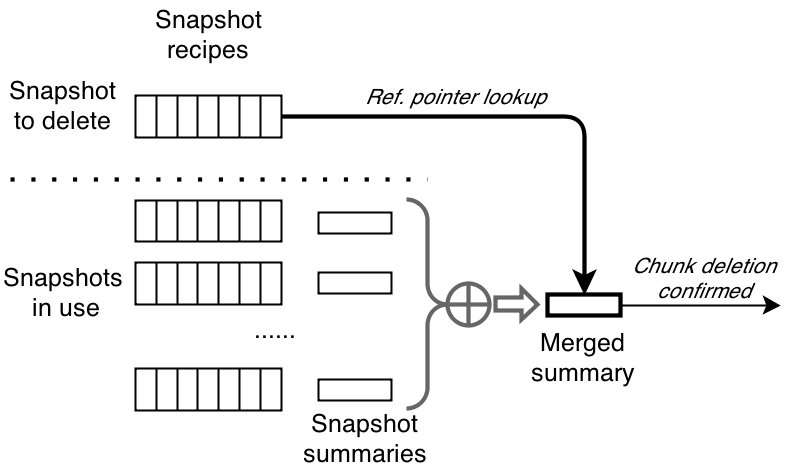
\epsfig{file=images/deletion.png, width=3.5in}
  \caption{Approximate deletion}
  \label{fig:deletion_flow}
\end{figure}

We design approximate deletion to fast identify unused data in the append store.
Instead of scanning the whold append store, it uses a bloom filter to check 
if a data are still referenced by living snapshots. However, there is a small false-positive probility which
would indetify unused data as in use, i.e., storage leakage.
The following steps would take place during an approximate deletion:

\begin{enumerate}
\item {\bf Creating bloom filter} Scan all the living snapshot recipess and their segment recipes,
for every reference pointing to append store, add it to the bloom filter.
\item {\bf Check existance} For every data reference in the deleted snapshot recipe and its segment recipes,
check the existance of that data reference in bloom filter. If not found, it is safe to delete that piece of data from append store
because no living snapshots has referenced it.
\end{enumerate}

The overall time of running a approximate deletion for one snapshot deletion would be scanning
all the living snapshots and deleted snapshots, since operations on the in-memory bloom filter can be done in
parallel and is much faster than loading recipes from DFS:
\begin{equation}
T = (N_{SS} + 1) * T_{scan\_recipes}
\end{equation}
 
Using the example and analysis in previous section, this approximate deletion can be done in 5 minutes. 
Memory usage of the bloom filter depends on its false-positive probility $P_{bl}$,
when set $P_{bl}$ to 0.01, the memory footprint of approximate deletion is about 15 MB.

The design goal of approximate deletion is to reduce the frequency of running accurate deletion.
For one VM's snapshots, let $D_{leakage}$ be the amount of storage leakage, $D_{del}$ be the average amount of data
to be deleted in one snapshot deletion, 
then we have:
\begin{equation}
D_{leakage} = N_{approximate} * P_{bl} * D_{del}
\end{equation}
where $N_{approximate}$ is the number of runs of approximate deletion. 
An accurate deletion is triggered to fix the storage leakage
when $D_{leakage}/D_{del}$ is accmulated to exceed certain threshold $T$:
\begin{equation}
D_{leakage} / D_{del} = N_{approximate} * P_{bl} > T \Rightarrow N_{approximate} > T/P_{bl}
\end{equation}
Therefore, when $P_{bl} = 0.01$ and $T=1$, 
there would be a run of accurate deletion for every $T/P_{bl} = 100$ runs of approximate deletion.
On a machine that hosts 20 VMs and each VM deletes snapshot daily, there would be less than
one accurate deletion scheduled per day.

\subsection{Accurate Deletion}
Our accurate deletion uses mark-and-sweep to find all the unused chunks in a VM's append store.
The following steps would take place during an accurate deletion:

\begin{enumerate}
\item Scan all the containers. For each container, extract full list of existing data references and allocate a bitmap. 
(Notice this list is self sorted.)
\item Scan all the snapshot recipes and segment recipes. For every data reference pointing to append store,
find it in the above lists and mark the corresponding position in bitmaps.
\item Scan the bitmaps, for every bit that are not marked, tell append store the corresponding data reference can be deleted.
\end{enumerate}

Although accurate deletion guarantees reliability and correctness, its speed and resource usage are big problems to our VM cloud.
Let $T_{scan\_AS}$ be the time to scan the VM's append store, $T_{scan\_recipes}$ be the time to scan one snapshot recipe
and its segment recipes, $T_{mark}$ be the time of finding a data reference in the list and mark bitmap, 
$N_{SS}$ be the number of snapshots and $N_c$ be the number of chunks in one snapshot.
The overall time of running an accurate deletion for one VM is:
\begin{equation}
T = T_{scan\_AS} + N_{SS} * T_{scan\_recipes} + N_{SS} * N_c * T_{mark}
\end{equation}

For a virtual disk that has 10 snapshots, 50 GB of data in the append store, $T_{scan\_AS}$ would have cost half an hour already.
In addition, scanning recipes of 10 snapshots cost another 5 minutes.
Furthermore, maintaining the full lists of data references and bitmaps costs about 100 MB of memory. Having tens of VMs
co-lived in one physical machine and deleting snapshot on a daily basis, 
it's infeasible to run accurate deletion as frequent as snapshot deletions.

\subsection{Discussion}

%\subsubsection{Fault Analysis }

We  compare the impact of losing $d$ machines using the following two approaches:
\begin{itemize}
\item The VM-centric approach (VC).  The replication degree of the backup storage 
is $r$ for regular content blocks and $r_c$ for CDS blocks where $r_c>r$. 
\item The VM-oblivious (VO) approach.
All chunk  blocks are treated uniformly and global comparison is conducted.
\end{itemize} 
 
When $d<r$, there is no loss of data in the snapshot storage.
When $d \ge r$, some of data blocks in the storage are loss, and we compute the number of VMs that could
suffer the loss of their snapshots.
We use the following parameters  during the analysis
\begin{itemize}
\item 	$V$ is the number of VMs. $m$ is the number of physical machines hosting the bakcup storage.
$d$ is the number of machines failed.
\item In the VC approach, $s_c$  of them in the backup storage
are shared by others with a zipf distribution. $(1-s_c)$ 
of them  is unique (nobody shares with them).
$L_c$ is the average number of VMs sharing a block (if it is in CDS for the VC approach.
$b_c$ is the number of shared blocks in VC.
\item In the VO approach, $s_o$ is the number of blocks shared.
$L_o$ is the average number of VMs sharing a block. 
\item $b$ is the  number of blocks stored in the storage after deduplication.
 \end{itemize}

The distribution of data blocks shared among VMs in VC follows a zipf distribution.
Given a VM block, the probability of being rank $x$ block is $P(x) = P(1) * x^{-\alpha}$
where $P(1)$ is the probability of being rank 1 most popular block.
Since $\sum P(x)= 1$, $P(1)= \frac{1}{\sum_1^{b_c} x^{-\alpha} }$.
Let $y$ be the number of VMs sharing rank $x$ block in VC, and  then  $y= V* P(x)$.

Thus the average number of VMs sharing a data block in the VC backup storage is:
\begin{equation}
%\begin{align}
\begin{split}
L_c& =  (1-s_c)*1 + s_c \sum_1^{b_c} P(x) * y \\
& =  (1-s_c)*1 + s_c \sum P(1)^2 *  x^{-2\alpha} *  V.
\end{split}
%\end{align}
\end{equation}

We can build a bipartite graph representing the association from unique data blocks
to their corresponding VMs. An association edge is  drawn  from a data block  to a VM 
if this block is used by this VM, 
The average incoming degree of VM nodes is equal to
the average outgoing degree of data blocks, which is $L_c$. 

\comments{
\begin{figure}[htbp]
\centering
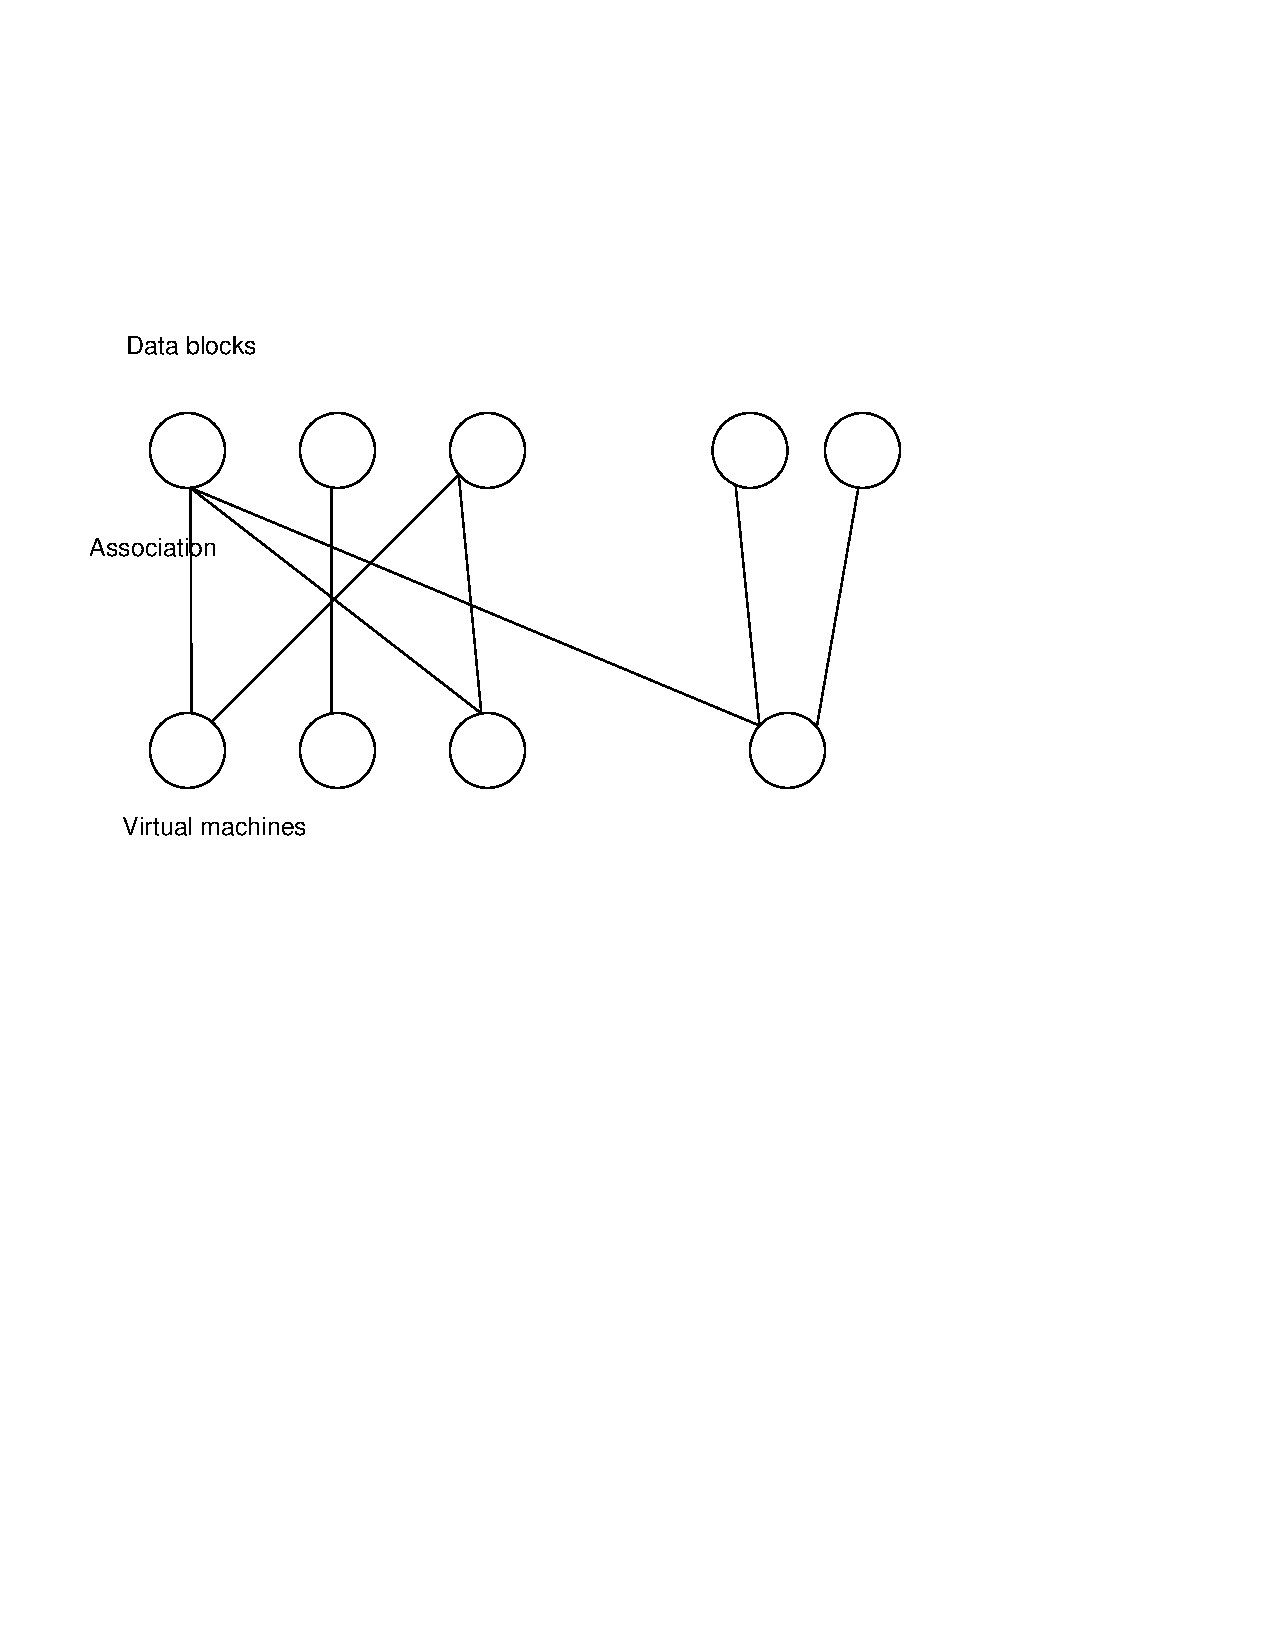
\includegraphics[width=0.45\textwidth]{shared.pdf}
\caption{Assoication of data blocks to VMs.}
\label{fig:shared}
\end{figure}
}

Under $d$ failed machines, the  expected number of VMs 
which suffer from data loss in VC is
\begin{multline}
%\begin{split}
 \sum_{1}^{V}  ( Probability (\mbox{ a VM fails)}) \\
= \sum_{1}^{V}  ( 1- Probability (\mbox{ a VM has no data loss)}) \\
= V ( 1-  Probability(\mbox{ A block has no data loss} )^{L_c} ).
%\end{split}
\end{multline}

\comments{
Prob(i-th block shared by (V-i+1) machines = X/i.
b
Sum (X/i) =1.      Thus       X= 1/ ln (V).
Length of sharing=  Probality(this block is shared with 1 VM) 1 + Probablity(this block shared by 2 VM) 2+..] =  X *V +X*(V-1)/2+ X*(V-2)/3 +..
=  X * sum (V-i+1)/I   for I from 1 to V.
=  (V+1) sum (X/i) . Sum(X) =  (V+1) -  X*V= V(1- 1/lnV) +1.
}

%Thus the number of VMs using a block =    $(1-s_c)  + s_c *L$.

When there are $d$ machines failed and the probability of
a block failure depends on if all replicas of this block reside in the failed machines.
When $r< d <r_c$,  only unshared data blocks can fail in VC. Then
%Probablity(\mbox { no loss for this  block}) = 1 - Probability (\mbox{ this block in d failed machiens})
\begin{multline}
%\begin{split}
Probability(\mbox{ A block has data loss})\\
= (1-s_c) (1- Probability (\mbox{ this block in d failed machines}))\\
= (1-s_c) (1- \frac{ \binom{d}{r}} { \binom{m}{r} }).
%\end{split}
\end{multline}
When $r_c \leq d$, shared data blocks in VC can have a loss. 
\[
Probability(\mbox{A block has data loss})
= 
(1-s_c) (1- \frac{ \binom{d}{r}} { \binom{m}{r} })
+ s_c (1- \frac{ \binom{r_c}{d}} { \binom{m}{r_c} }).
\]

By comparison, under $d$ failed machines, the  expected number of VMs 
which suffer from data loss in VO is
\[
V ( 1-  (1- \frac{ \binom{d}{r}} { \binom{m}{r} })^{L_o} ).
\]
where
\[
L_o = (1-s_o) + s_o \sum_1^b  P(1)^2 *  (x')^{-2\alpha'} *V.  
\]


\comments{
	=  sum _for_all_block(   Probablity (a block fails) *number of VM sharing this block ))
               = Probability(a block fails) * sum_for_all_blocks (numb of VM shared)
	= Probablity (a block fails) *b *aveageLengthVM
	= [ 1-  C(r, k) /C(n,r)] * b* [ 1+ s *V(1-1/ln V)]
  
----------------------------------------------------------------------       

For CDS model, 85% blocks are using the data from the same VM while upto 10% data is for CDS (we actually only use 5% perhaps).  Thus the overall speaking, at most 10% of data are shared.
Thus  for CDS approach,   the # VM failure caused by k machines is at most  [ 1-  C(r, k) /C(n,r)] * b* [ 1+ 0.10 *V(1-1/ln V)].
For original approach,  [ 1-  C(r, k) /C(n,r)] * b* [ 1+ 0.90 *V(1-1/ln V)].
For large V, the reliability improves by 9 times.
}

\section{Experiments}
Our main test-bed is an cluster of 6 machines,
each of which is equiped with a 8-core AMD FX-8120 at 3.1 GHz
with 16 GB RAM, running Linux.
A distributed file system (QFS) runs in the cluster manages six 3TB disks
 with default replication degree set to 3.
Our data set consists of 350 virtual machine image snapshots taken from Alibaba.com's
public VM cloud in China. We select 35 VMs from the most popular 7 OSes: 
Debian, Ubuntu, Redhat, CentOS, Win2003 32bit, win2003 64 bit and win2008 64 bit. 
For each OS, 5 VMs are chosen, and every VM come with 10 full snapshots.

\subsection{Replication cost}
\begin{table}
    \begin{tabular}{|c|c|}
    \hline
    PDS replication degree & Total space (GB) \\ \hline
    3                      & 3065             \\ \hline
    4                      & 3072             \\ \hline
    5                      & 3079             \\ \hline
    6                      & 3086             \\ \hline
    7                      & 3093             \\ \hline
    \end{tabular}
\caption{Storage space cost under different PDS replication degree}
\label{tab:replcation_cost}
\end{table}

\subsection{System Performance}
{\bf Single VM Backup} We start the evauluation of our system by examine the normal warmed-up
backup scenario - taking a snapshot of a VM which already has old backups exist. To simulate this
scenario, we pick one 40GB VM from the data set, make an initial snapshot backup, then
evaulate the system performance on the second snapshot backup. We repeat such procedure
under different CDS memory usage settings, the results of backup time break down are shown in
firure~\ref{fig:single_vm_backup}. 

It's easy to see that the time of I/O dominates the backup process, our deduplication
procedure only takes a tiny fraction of the total backup time. Larger memory permits us to
use larger CDS index to cover more of global index, as a result the amount of data to be writen
is reduced and so do the writing time.
Inside the deduplication procedure, the time costs of level-1
is plainly zero, and the costs of level-2 and level-3 are almost identical under different settings
because the number of fingerprints to process are just the same.

{\bf Parallel VM Backup} We then evaluate the performance of writing snapshots in parallel.
To begin, on each node we let 4 VMs writing snapshot concurrently, and gradually 
increase number of VMs to 12 to saturate our system capability. We observed 
the per-node throughput peaked at 2700 MB/s when writing 10 VM snapshots in parallel, 
which is far beyond our QFS file system capability. The reason behind it is our efficient
deduplication architecture and compression greatly reduce the amount of data that need to be writen to
the file system. The main bottleneck here is our QFS only manages one disk per node, 
making it inefficient to utilize the benefits of parallel disk access. We expect our achitecture can
perform even better in production cluster which normally has more than ten disks on each node.

\begin{figure}
    \centering
    \subfigure[Real VM backup performance]
    {
        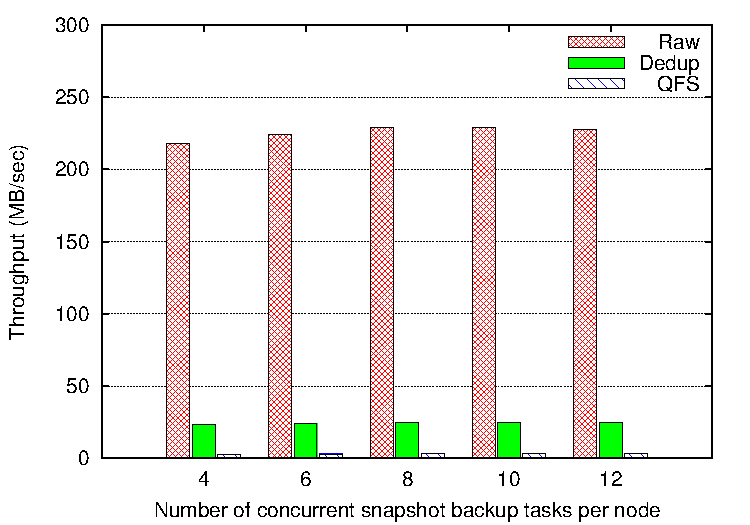
\includegraphics[width=3in]{figures/parallel_backup_with_read.pdf}
        \label{fig:withread}
    }
    \\
    \subfigure[Deduplication and storage system performance]
    {
        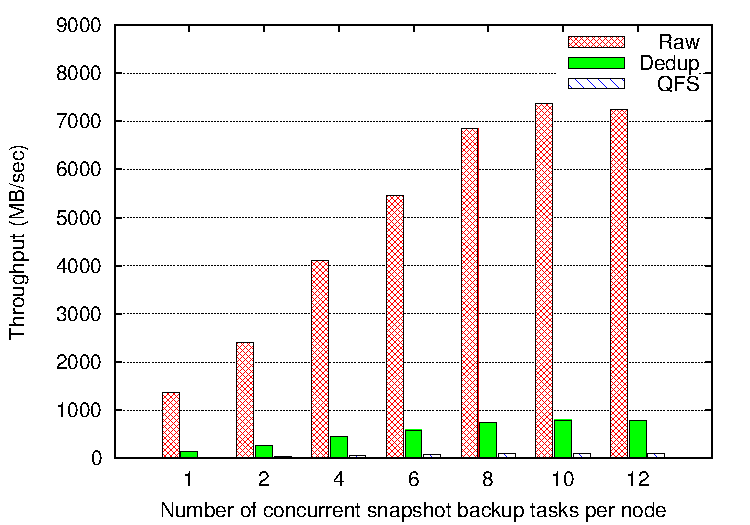
\includegraphics[width=3in]{figures/parallel_backup_no_read.pdf}
        \label{fig:noread}
    }
    \caption{Throughput per-node with concurrent snapshot backup tasks}
    \label{fig:parallel_backup}
\end{figure}

\begin{figure}[htbp]
  \centering
  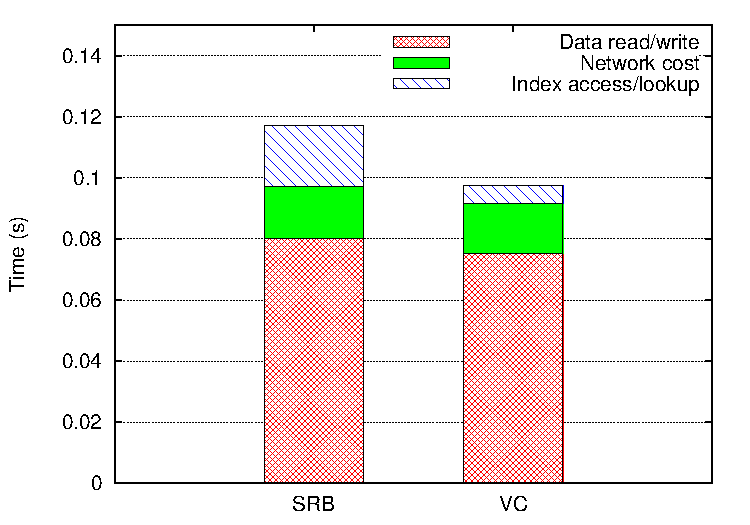
\epsfig{file=figures/srb_vs_vc.pdf, width=3.5in}
  \caption{Time to backup a dirty segment under SRB and VC approach}
  \label{fig:srb_vs_vc}
\end{figure}




% \begin{figure}[htbp]
%   \centering
%   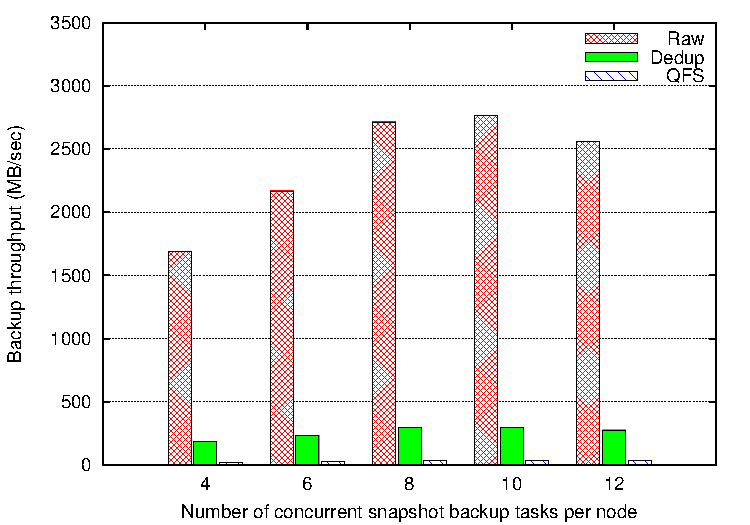
\epsfig{file=figures/parallel_backup.pdf, width=3.5in}
%   \caption{Throughput per-node with concurrent snapshot backup tasks}
%   \label{fig:parallel_backup}
% \end{figure}


% \begin{table}
% \begin{tabular}{ |p{1.5cm}|p{1.8cm}|p{1.2cm}|p{1.4cm}| }
% \hline
%  & Costs & Stateless routing with binning (s) & VM-centric approach (s) \\ \hline
% \multirow{4}{*}{\vbox{I/O related}} & Read data & 0.05 & 0.05 \\ \cline{2-4}
%  & Transfer data  & 0.017 & 0.017 \\ \cline{2-4}
%  & Write data & 0.03 & 0.025 \\ \cline{2-4}
%  & Subtotal & 0.097 & 0.092 \\ \hline
% \multirow{5}{*}{\vbox{Dedupe related}} & Read index/recipe & 0.01 & 0.00045 \\ \cline{2-4}
%  & Write index/recipe & 0.01 & 0.0051 \\ \cline{2-4}
%  & Transfer fingerprints & 0.00058 & 0.00013 \\ \cline{2-4}
%  & CDS lookup & N/A & 0.00034 \\ \cline{2-4}
%  & Subtotal & 0.021 & 0.0064 \\ \hline
% \multicolumn{2}{ |c| }{Total} & 0.12 & 0.098 \\
% \hline
% \end{tabular}
% \caption{Time of backup a segment break down}
% \label{tab:compare}
% \end{table}


\subsection{Comparison with Other Approaches}
\subsubsection{Extreme Binning}
%\comments{
    %this version of the figure is vertical
    \begin{figure}[ht]
  \centering
    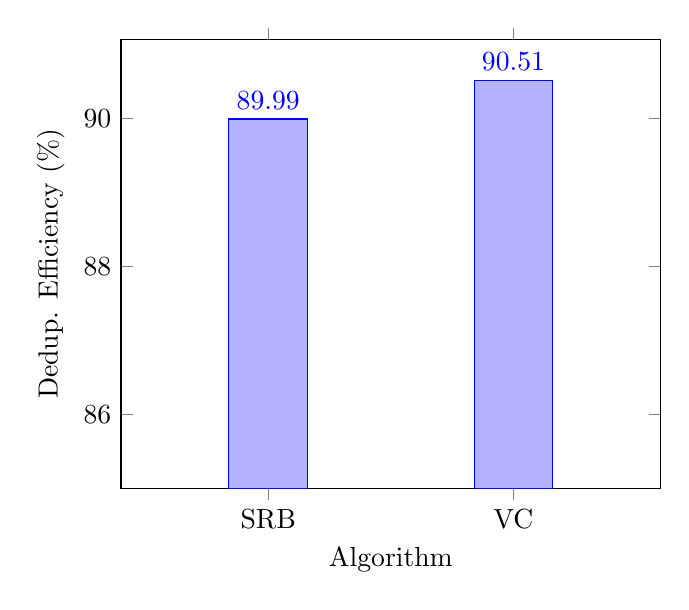
\begin{tikzpicture}
            \begin{axis}[
            %title={Extreme-Binning Efficiency},
            ybar,
            bar width=1.00cm,
            symbolic x coords={SRB,VC},
            xlabel={Algorithm},
            ylabel={Dedup. Efficiency (\%)},
            %extra y ticks={4.5,5.5,6.5} %to add extra ticks
            xtick=data, %without this the symbolic coords may be repeated as filler
            enlarge x limits=0.6, %used to push plots towards center
            ymin=85,
            %ymax=100,
            nodes near coords,
            nodes near coords align={vertical},
            ]
            \addplot coordinates {(SRB,89.99) (VC,90.51)};
            \end{axis}
    \end{tikzpicture}
    \caption{Deduplication Efficiency
        ($efficiency=\frac{d-du}{d-du_{complete}}$) comparison between Stateless Routing with Binning and VC with 2\% CDS.}
  \label{fig-exbin-efficiency}
\end{figure}
%}
%same figure as above but horizontal (better for only two data points)
\begin{figure}[ht]
  \centering
    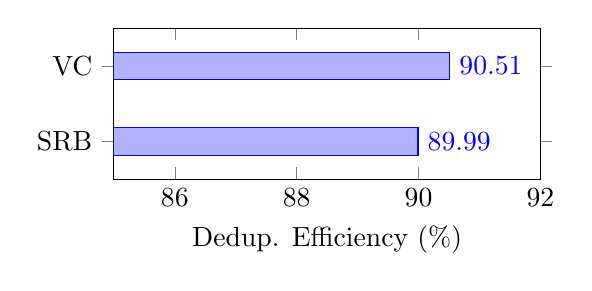
\begin{tikzpicture}
            \begin{axis}[
            %title={Extreme-Binning Efficiency},
            xbar,
            width=7cm,
            height=3.5cm,
            %bar width=0.75cm,
            symbolic y coords={SRB,VC},
            xlabel={Dedup. Efficiency (\%)},
            %ylabel={Algorithm},
            %extra x ticks={4.5,5.5,6.5} %to add extra ticks
            ytick=data, %without this the symbolic coords may be repeated as filler
            enlarge y limits=0.5,
            xmin=85,
            xmax=92, %otherwise label overlaps with right border
            nodes near coords,
            nodes near coords align={horizontal},
            ]
            \addplot coordinates {(89.99,SRB) (90.51,VC)};
            \end{axis}
    \end{tikzpicture}
    \caption{Deduplication Efficiency
        ($efficiency=\frac{d-du}{d-du_{complete}}$) comparison between Stateless Routing with Binning and VC with 2\% CDS.}
  \label{fig-exbin-efficiency}
\end{figure}

%graph comparing extreme binning (SRB) with CDS model (VC) for different cds percentages
\begin{figure}[ht]
  \centering
    \begin{tikzpicture}
            \begin{axis}[
            %title={Ex-Binning Efficiency},
            xlabel={Number of VMs added},
            ylabel={Dedup. Efficiency (\%)},
            %extra y ticks={4.5,5.5,6.5} %to add extra ticks
            mark options=solid,
            legend pos=south west,
            %legend columns=2,
            %legend style={
            %    at={(0.5,-0.2)},
            %anchor=north}
            ]
            \addplot[color=blue,mark=none] table[x=VMs,y=exbin] {figures/exbin_efficiency_comparison.txt};
            \addplot[densely dotted, color=red,mark=none] table[x=VMs,y=cds1] {figures/exbin_efficiency_comparison.txt};
            \addplot[loosely dotted, color=brown,mark=none] table[x=VMs,y=cds2] {figures/exbin_efficiency_comparison.txt};
            \addplot[densely dashed,color=black,mark=none] table[x=VMs,y=cds4] {figures/exbin_efficiency_comparison.txt};
            \legend{SRB,VC (1\%CDS),VC (2\%CDS),VC (4\%CDS)};
            \end{axis}
    \end{tikzpicture}
    \caption{Deduplication Efficiency
        ($efficiency=\frac{d-du}{d-du_{complete}}$) comparison between
    Stateless Routing with Binning and VC.}
  \label{fig-exbin-efficiency-graph}
\end{figure}


\comments{
\subsection{Read Snapshot}

\subsection{Comparison with Other Approaches}
\subsubsection{Sampled Index}
One alternative approach to avoiding a single global index is to use a sampled
index. This is the approach taken by Guo and Efstathopoulos\cite{Guo2011}. We
compare their solution to ours by running their algorithm on our 350 traces
using a sampling rate of 1 out of 101 blocks, and always including the first
block in a container (which we fix at 16MB in size). The results of running this
test are shown in Table~\ref{??}, and the memory usage comparison can be found
Sec.~\ref{??}. Our results show that using a sampled index achieves a very high
rate of deduplication, and so a sampled index might be a good way to do dedup
in a single node setup.

The problems for sampling are in distributing the
algorithm and in deduplicating extremely large bodies of data. The algorithm
stores the entire (sampled) index in memory, which is required for high
throughput to avoid the disk-bottleneck problem - since the index itself has no
locality information, lookups are essentially random, so the index must be
somehow optimized to prevent excessive disk seeking (the sampling algorithm does
this by storing the index in memory). To distribute this index, each node would
either require a complete copy of the index which would have a prohibitive cost in
memory, or something like memcached must be used, which leaves the same problem
as the disk bottleneck with every index check potentially using the network.
The difficulty in storing extremely large bodies of data
is related, as once 1PB is stored in the system, assuming a sampling rate of 
1/101 with 22 byte index entires, 55GB of (in memory) index are required.

Our solution uses more total memory (??how much??), but is more scalable both in
terms of capactity and distributing the deduplication. The only part of our
algorithm which requires significant network traffic is the CDS deduplication,
but this is done after Levels 1 and 2 (dirty bits and comparison to parent), and
so is only done for a small percent of blocks (?? 5-10\% ??).

\subsubsection{Scalable Data Routing}
Another approach to avoiding a global index is to use a content-based hash
partitioning algorithm to break up the deduplication work. This approach is
taken by Dong et al. in their Scalable Data Routing paper, and is similar to
Exreme Binning\cite{??}\cite{extreme_binning09}. We compared our solution to
content-based hash partitioning by running the algorithm on our set of 
traces. We used 2MB superchunks and 4KB chunks to partition the data, and use
the minhashes of the superchunks for routing. The results of this are shown in
Table~\ref{??}. Routing each chunk to a bin provides good deduplication
efficiency, and only requires each storage node to keep an index of local data
and the bin mapping, but misses significant opportunities in our indended use
case.

The problem with the Data Routing algorithm is in the very high network traffic.
Our intended use case is a backup system which runs alongside a number of VMs,
in order to save costs. Data Routing makes no use of the inherent locality in
such a system, and therefore puts a much higher network burden on machines which
are also running 35 VMs each. This will reduce the available network bandwidth
to users of the VMs, and/or reduce the possible deduplication throughput.

}

\section{Conclusion}
\label{sect:final}
In this paper we propose a VM-centric deduplication scheme for 
VM snapshot backup in the cloud for maximizing fault isolation and tolerance. 
Inner-VM deduplication localizes backup data dependency and exposes more parallelism  
while cross-VM deduplication with a small common data set
effectively  covers a large percent of duplicate data.
The scheme organizes the write of small data chunks into large file system blocks so
that each underlying file block is associated with one VM for most cases.
by keeping most of the FSBs only referenced by 1 VM, we isolate faults and improve overal fault tolerance.
Our solution accomplishes reasonable and competitive deduplication efficiency while
still meeting stringent cloud resource usage requirements. 
Our analysis shows that  this VM centric scheme 
can  provide  better fault tolerance than VM-oblivious global deduplication schemes
while using a small amount of computing and storage resources. 


[Talk about more what we learn from Evaluation]
Evaluation using real user's VM data shows
our solution can accomplish 92\% of what complete global
deduplication can do. 
Compare to today's widely-used snapshot technique, our scheme reduces almost
two-third of snapshot storage cost.
Finally, our scheme uses a very small amount of memory on each node, and leaves
room for additional optimization we are further studying.


%This paper studies a cluster-based VM-centric scheme which collocates a lightweight
%backup service with the cloud service and it integrates multiple duplicate detection strategies that  
%localize the deduplication as much as possible within each virtual machine.
%This  paper  provides a comparative evaluation of this scheme in  accomplishing a high deduplication 
%efficiency while sustaining a good backup throughput. 

%This paper studies the      a VM snapshot storage architecture which adopts multiple-level selective deduplication to bring the benefits of fine-grained data reduction into cloud backup storage systems.
%In this work, we describe our working snapshot system implementation, and provide
%early performance measurements for both deduplication impact and
%snapshot operations.

\comments{
\section*{Acknowledgments}
{
We would like to thank Weicai Chen and Shikun Tian from Alibaba for their kind support, 
and the anonymous referees for their comments.
Wei Zhang has received internship support from Alibaba  for VM backup system development.
This work was supported in part by NSF IIS-1118106.
Any opinions, findings, and conclusions or recommendations expressed in this material are those of the authors and
do not necessarily reflect the views of Alibaba or the National Science Foundation.
}
}
%Noted that 6\% is still significant, which is about 24GB per each VM and for a 1000 node Aliyun cluster,
%this is about 600 terabytes.
 
%Our experiments show th
%our solution can eliminate the majority of data duplication with a tiny fraction of
%block hash index store in memory. It does not only saves valuable system resouces in
%the VM cloud, but also makes deduplication much faster.
%
%
%Using  50 user VM data out of 1322 data disks as the training data and
%with  1.5\% as PDS threshold, we see the total 1198GB of new data is reduced by
%755.8GB, while perfect deduplication can reduce 1017.4GB. So 74.3\% of duplicate blocks are eliminated
%by pre-trained PDS, which is quite satisfactory.



\bibliographystyle{abbrv}
\bibliography{library}
\end{document}
